\documentclass[a4paper,11pt,twoside]{report}
% KOMPILOWAĆ ZA POMOCĄ pdfLaTeXa, PRZEZ XeLaTeXa MOŻE NIE BYĆ POLSKICH ZNAKÓW

% -------------- Kodowanie znaków, język polski -------------

\usepackage[utf8]{inputenc}
\usepackage[MeX]{polski}
\usepackage[T1]{fontenc}
\usepackage[english,polish]{babel}

\usepackage{amsmath, amsfonts, amsthm, latexsym} % głównie symbole matematyczne, środowiska twierdzeń

\usepackage[final]{pdfpages} % inputowanie pdfa
%\usepackage[backend=bibtex, style=verbose-trad2]{biblatex}
\usepackage{url}

% ---------------- Marginesy, akapity, interlinia ------------------

\usepackage[inner=20mm, outer=20mm, bindingoffset=10mm, top=25mm, bottom=25mm]{geometry}

\usepackage{float}
\linespread{1.5}
\allowdisplaybreaks

\usepackage{indentfirst} % opcjonalnie; pierwszy akapit z wcięciem
\setlength{\parindent}{5mm}

%--------------------------- Tabele -----------------------------
\usepackage{longtable}
\usepackage{makecell}
\renewcommand{\tablename}{Tabela}



%--------------------------- ŻYWA PAGINA ------------------------

\usepackage{fancyhdr}
\pagestyle{fancy}
\fancyhf{}
% numery stron: lewa do lewego, prawa do prawego 
\fancyfoot[LE,RO]{\thepage} 
% prawa pagina: zawartość \rightmark do lewego, wewnętrznego (marginesu) 
\fancyhead[LO]{\sc \nouppercase{\rightmark}}
% lewa pagina: zawartość \leftmark do prawego, wewnętrznego (marginesu) 
\fancyhead[RE]{\sc \leftmark}

\renewcommand{\chaptermark}[1]{
\markboth{\thechapter.\ #1}{}}

% kreski oddzielające paginy (górną i dolną):
\renewcommand{\headrulewidth}{0 pt} % 0 - nie ma, 0.5 - jest linia


\fancypagestyle{plain}{% to definiuje wygląd pierwszej strony nowego rozdziału - obecnie tylko numeracja
  \fancyhf{}%
  \fancyfoot[LE,RO]{\thepage}%
  
  \renewcommand{\headrulewidth}{0pt}% Line at the header invisible
  \renewcommand{\footrulewidth}{0.0pt}
}



% ---------------- Nagłówki rozdziałów ---------------------

\usepackage{titlesec}
\titleformat{\chapter}%[display]
  {\normalfont\Large \bfseries}
  {\thechapter.}{1ex}{\Large}

\titleformat{\section}
  {\normalfont\large\bfseries}
  {\thesection.}{1ex}{}
\titlespacing{\section}{0pt}{30pt}{20pt} 
%\titlespacing{\co}{akapit}{ile przed}{ile po} 
    
\titleformat{\subsection}
  {\normalfont \bfseries}
  {\thesubsection.}{1ex}{}


% Dodawanie pdfów
\usepackage{pdfpages}

% ----------------------- Spis treści ---------------------------
\def\cleardoublepage{\clearpage\if@twoside
\ifodd\c@page\else\hbox{}\thispagestyle{empty}\newpage
\if@twocolumn\hbox{}\newpage\fi\fi\fi}


% kropki dla chapterów
\usepackage{etoolbox}
\makeatletter
\patchcmd{\l@chapter}
  {\hfil}
  {\leaders\hbox{\normalfont$\m@th\mkern \@dotsep mu\hbox{.}\mkern \@dotsep mu$}\hfill}
  {}{}
\makeatother

\usepackage{titletoc}
\makeatletter
\titlecontents{chapter}% <section-type>
  [0pt]% <left>
  {}% <above-code>
  {\bfseries \thecontentslabel.\quad}% <numbered-entry-format>
  {\bfseries}% <numberless-entry-format>
  {\bfseries\leaders\hbox{\normalfont$\m@th\mkern \@dotsep mu\hbox{.}\mkern \@dotsep mu$}\hfill\contentspage}% <filler-page-format>

\titlecontents{section}
  [1em]
  {}
  {\thecontentslabel.\quad}
  {}
  {\leaders\hbox{\normalfont$\m@th\mkern \@dotsep mu\hbox{.}\mkern \@dotsep mu$}\hfill\contentspage}

\titlecontents{subsection}
  [2em]
  {}
  {\thecontentslabel.\quad}
  {}
  {\leaders\hbox{\normalfont$\m@th\mkern \@dotsep mu\hbox{.}\mkern \@dotsep mu$}\hfill\contentspage}
\makeatother



% ---------------------- Spisy tabel i obrazków ----------------------

\renewcommand*{\thetable}{\arabic{chapter}.\arabic{table}}
\renewcommand*{\thefigure}{\arabic{chapter}.\arabic{figure}}
%\let\c@table\c@figure % jeśli włączone, numeruje tabele i obrazki razem


% --------------------- Definicje, twierdzenia etc. ---------------


\makeatletter
\newtheoremstyle{definition}%    % Name
{3ex}%                          % Space above
{3ex}%                          % Space below
{\upshape}%                      % Body font
{}%                              % Indent amount
{\bfseries}%                     % Theorem head font
{.}%                             % Punctuation after theorem head
{.5em}%                            % Space after theorem head, ' ', or \newline
{\thmname{#1}\thmnumber{ #2}\thmnote{ (#3)}}%  % Theorem head spec (can be left empty, meaning `normal')
\makeatother

% ----------------------------- POLSKI --------------------------------

\theoremstyle{definition}
\newtheorem{theorem}{Twierdzenie}[chapter]
\newtheorem{lemma}[theorem]{Lemat}
\newtheorem{example}[theorem]{Przykład}
\newtheorem{proposition}[theorem]{Stwierdzenie}
\newtheorem{corollary}[theorem]{Wniosek}
\newtheorem{definition}[theorem]{Definicja}
\newtheorem{remark}[theorem]{Uwaga}



% ----------------------------- Dowód -----------------------------

%\makeatletter
%\renewenvironment{proof}[1][\proofname]
%{\par
%  \vspace{-12pt}% remove the space after the theorem
%  \pushQED{\qed}%
%  \normalfont
%  \topsep0pt \partopsep0pt % no space before
%  \trivlist
%  \item[\hskip\labelsep
%        \sc
%    #1\@addpunct{:}]\ignorespaces
%}
%{%
%  \popQED\endtrivlist\@endpefalse
%  \addvspace{20pt} % some space after
%}
%
%\renewcommand{\qedhere}{\hfill \qedsymbol}
%\makeatother





% -------------------------- POCZĄTEK --------------------------


% --------------------- Ustawienia użytkownika ------------------

\newcommand{\tytul}{System obliczeń rozproszonych z węzłami działającymi w przeglądarce internetowej}
\renewcommand{\title}{A system for distributed computing with web browser--based nodes}
\newcommand{\type}{inżyniers} % magisters, licencjac
\newcommand{\supervisor}{mgr inż. Jan Karwowski}



\begin{document}
\sloppy


\includepdf[pages=-]{titlepage/titlepage}


% ------------------ STRONA Z PODPISAMI AUTORA/AUTORÓW I PROMOTORA ------------------


\thispagestyle{empty}\newpage
\null

\vfill

\begin{center}
\begin{tabular}[t]{ccc}

............................................. & \hspace*{100pt} & .............................................\\
podpis promotora & \hspace*{100pt} & podpis autora


\end{tabular}
\end{center}



% ---------------------------- ABSTRAKTY -----------------------------
% W PRACY PO POLSKU, NAPIERW STRESZCZENIE PL, POTEM ABSTRACT EN

{
\begin{abstract}

\begin{center}
\tytul
\end{center}

Streszczam.

Lorem ipsum dolor sit amet, consetetur sadipscing elit, sed diam nonumyeirmod tempor invidunt ut labore et dolore magna aliquyam erat, sed diamvoluptua. At vero eos et accusam et justo duo dolores et ea rebum. Stet clita kasd gubergren, no sea takimata sanctus est Lorem ipsum dolor sit amet.\\

\noindent \textbf{Słowa kluczowe:} obliczenia rozproszone, WebAssembly, aplikacja internetowa, wydajność, równoległość, przeglądarka internetowa, Internet
\end{abstract}
}

\null\thispagestyle{empty}\newpage

{\selectlanguage{english}
\begin{abstract}

\begin{center}
\title
\end{center}

Lorem ipsum dolor sit amet, consetetur sadipscing elitr, sed diam nonumyeirmod tempor invidunt ut labore et dolore magna aliquyam erat, sed diamvoluptua. At vero eos et accusam et justo duo dolores et ea rebum. Stet clita kasd gubergren, no sea takimata sanctus est Lorem ipsum dolor sit amet.

Lorem ipsum dolor sit amet, consetetur sadipscing elitr, sed diam nonumyeirmod tempor invidunt ut labore et dolore magna aliquyam erat, sed diamvoluptua. At vero eos et accusam et justo duo dolores et ea rebum. Stet clita kasd gubergren, no sea takimata sanctus est Lorem ipsum dolor sit amet.\\

\noindent \textbf{Keywords:} keyword1, keyword2, ...
\end{abstract}
}


% --------------------- OŚWIADCZENIE -----------------------------------------


\null\thispagestyle{empty}\newpage

\null \hfill Warszawa, dnia ..................\\

\par\vspace{5cm}

\begin{center}
Oświadczenie
\end{center}

\indent Oświadczam, że moją część pracy \type kiej (zgodnie z podziałem zadań opisanym w pkt TODO) pod
tytułem ,,\tytul '', której promotorem jest \supervisor , wykonałem
samodzielnie, co poświadczam własnoręcznym podpisem.
\vspace{2cm}


\begin{flushright}
  \begin{minipage}{50mm}
    \begin{center}
      ..............................................

    \end{center}
  \end{minipage}
\end{flushright}

\thispagestyle{empty}
\newpage

\null\thispagestyle{empty}\newpage


% ------------------- 4. Spis treści ---------------------
\pagenumbering{gobble}
\tableofcontents
\thispagestyle{empty}

\newpage % JEŻELI SPIS TREŚCI MA PARZYSTĄ LICZBĘ STRON, ZAKOMENTOWAĆ
% ALBO JAK KTOŚ WOLI WTEDY DWIE STRONY ODSTĘPU, DODAĆ \null\newpage

% -------------- 5. ZASADNICZA CZĘŚĆ PRACY --------------------
\null\thispagestyle{empty}\newpage
\pagestyle{fancy}
\pagenumbering{arabic}
\setcounter{page}{11} % JEŻELI Z POWODU DUŻEJ ILOŚCI STRON W SPISIE TREŚCI SIĘ NIE ZGADZA, TRZEBA ZMODYFIKOWAĆ RĘCZNIE

\chapter{Wstęp}
    Opis czego będzie dotyczyła praca inżynierska

\chapter{Analiza problemu}
    \section{Cel projektu}
        Opisanie, że aktualnie nie ma na rynku rozwiązań pozwalających na obliczenia rozproszone w przeglądarce.
    
    \section{Opis istniejących rozwiązań}
        Blazor, Bridge.NET, JSIL, inne frameworki do obliczeń rozproszonych
        Zaznaczenie, że my spinamy te rzeczy w jedno
        
    \section{Wymagania funkcjonalne}
        Jak na dokumentacji z PZ
        
    \section{Wymagania niefunkcjonalne}
        Jak na dokumentacji z PZ
    
\chapter{Architektura systemu}
 Zaprojektowany system składa się z trzech modułów:

\begin{itemize}
    \item Serwera
    \item Panelu administracyjnego
    \item Interfejsu dla węzłów obliczeniowych
\end{itemize}

Na rysunku~\ref{project-model} znajdują się wyodrębnione moduły wraz z urządzeniami podłączonymi do systemu.

Wszelkie interakcje pomiędzy modułami odbywają się z wykorzystaniem sieci Internet. Proxy rozdziela ruch między serwerem aplikacyjnym oraz serwerem udostępniającym interfejs użytkownika w przeglądarce (zarówno dla węzłów obliczeniowych, jak i administratora). Proxy akceptuje jedynie protokół HTTP (port \textit{80}). Protokół HTTPS (port \textit{443}) nie jest zapewniany w ramach przygotowanego systemu.


\begin{figure} \centering{
        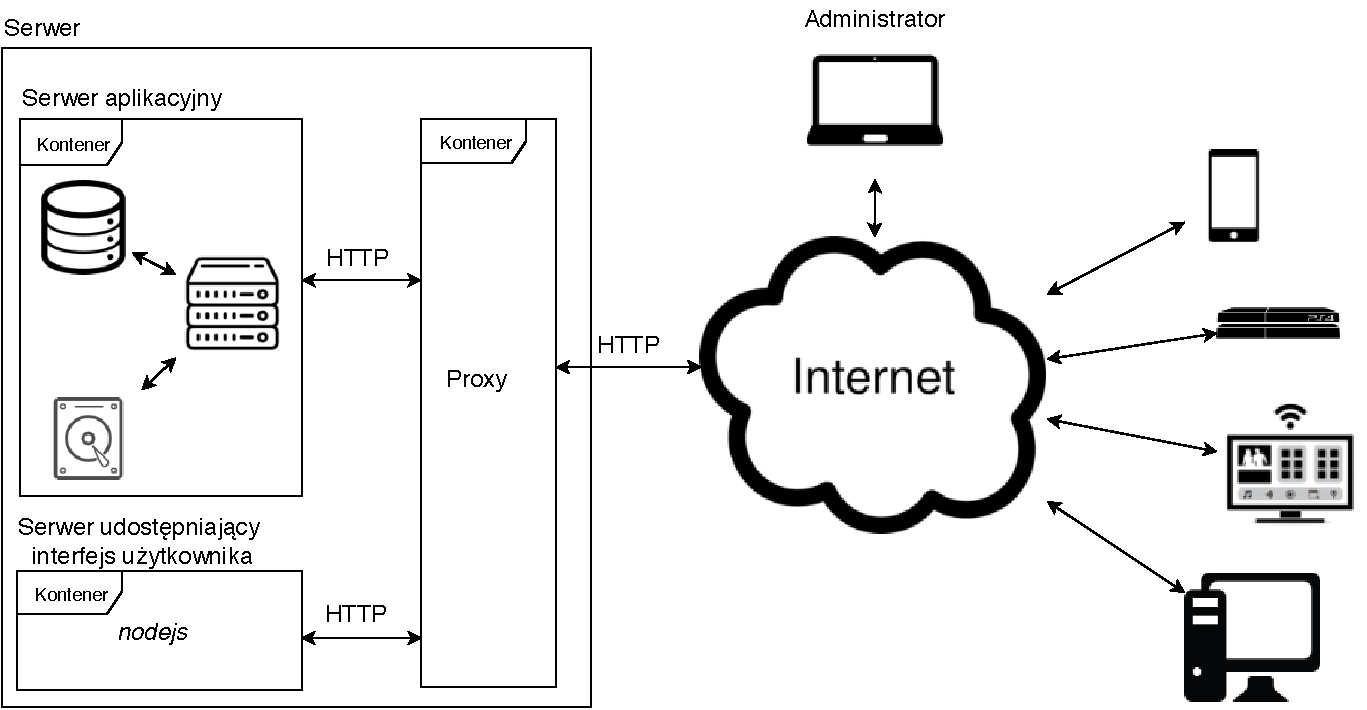
\includegraphics[scale=0.75]{images/project-model.pdf}}
    \caption{Moduły systemu.}
    \label{project-model}
\end{figure}

\section{Projekt modułów}

W tej sekcji znajdują się opisy poszczególnych modułów wraz z ich podziałem na składowe.

\subsection{Serwer}

Serwer stanowi główny komponent całego systemu obliczeń rozproszonych. Do jego zadań należy między innymi zarządzanie encjami w bazie danych, przygotowanie bibliotek utworzonych w \textit{.NET Standard 2.0}~\cite{dotnet-standard} do uruchomienia w \textit{WebAssembly}~\cite{webassembly} oraz dystrybucja zadań pomiędzy węzłami obliczeniowymi. Serwer udostępnia także API zgodne ze standardem \textit{JSON API}~\cite{jsonapi}.

Komponenty składowe serwera zostały przedstawione na rysunku~\ref{server-model}.

\begin{figure} \centering{
        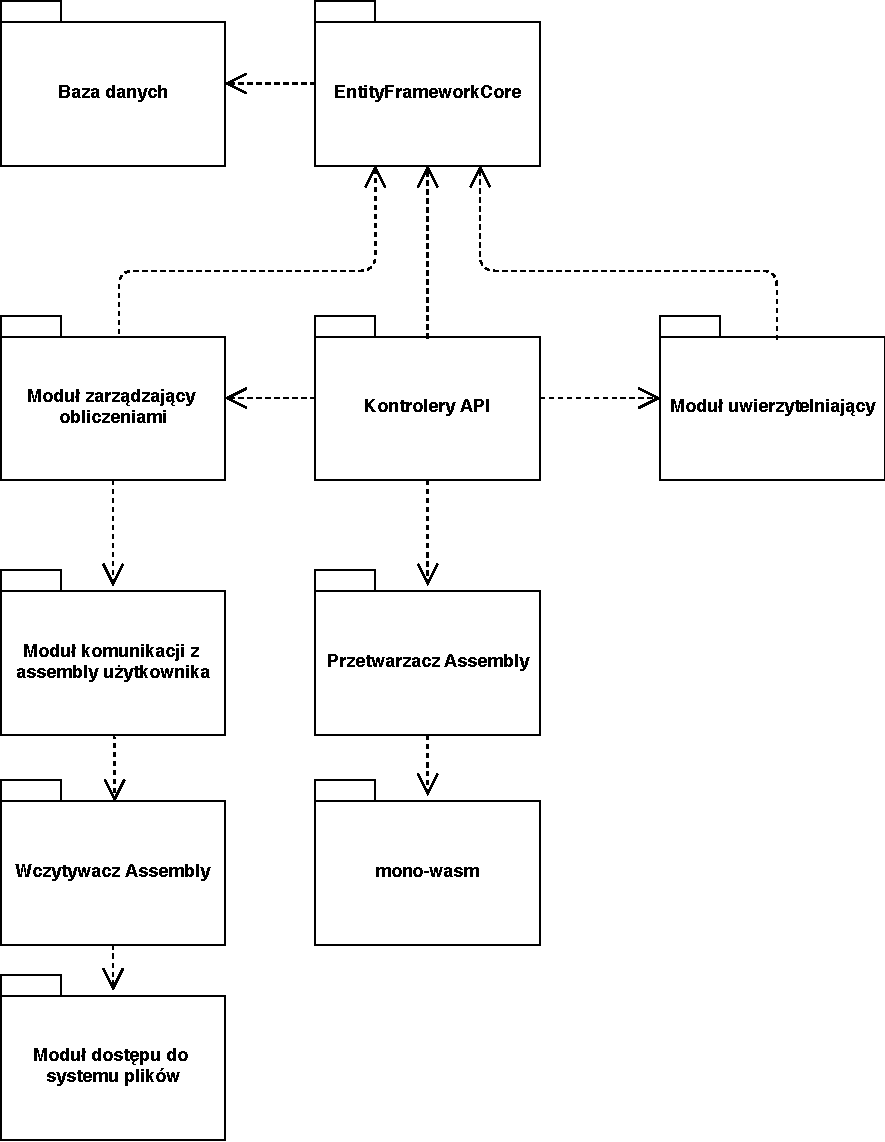
\includegraphics[scale=0.75]{images/moduly-serwera.pdf}}
    \caption{Moduły serwera.}
    \label{server-model}
\end{figure}

\subsection{Panel administracyjny}

Panel administracyjny umożliwia użytkownikom zarządzanie dodanymi bibliotekami oraz zadaniami za pomocą przejrzystego interfejsu użytkownika. Dostęp do tego modułu jest dostępny po uprzedniej autoryzacji za pomocą hasła. 

Komponenty, które tworzą panel administracyjny zostały przedstawione na rysunku~\ref{admin-panel-model}. 

\begin{figure} \centering{
        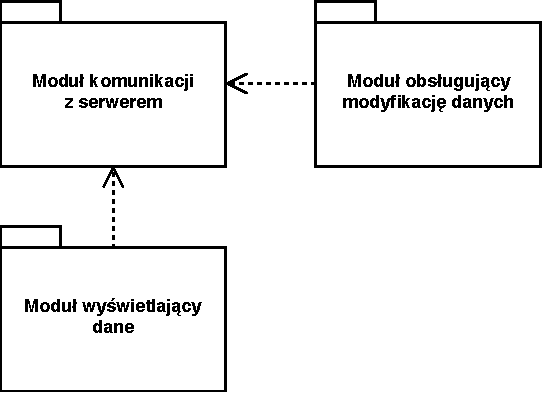
\includegraphics[scale=0.75]{images/moduly-panelu-administracyjnego.pdf}}
    \caption{Moduły panelu administracyjnego.}
    \label{admin-panel-model}
\end{figure}

\subsection{Węzły obliczeniowe}

Węzły obliczeniowe są odpowiedzialne za wykonywanie zadanych im obliczeń, a następnie zgłaszanie ich rezultatów. Węzeł obliczeniowy posiada również prosty interfejs graficzny pozwalający na zarządzanie jego pracą.

Podział węzłów obliczeniowych na moduły znajduje się na rysunku~\ref{node-model}.

\begin{figure} \centering{
        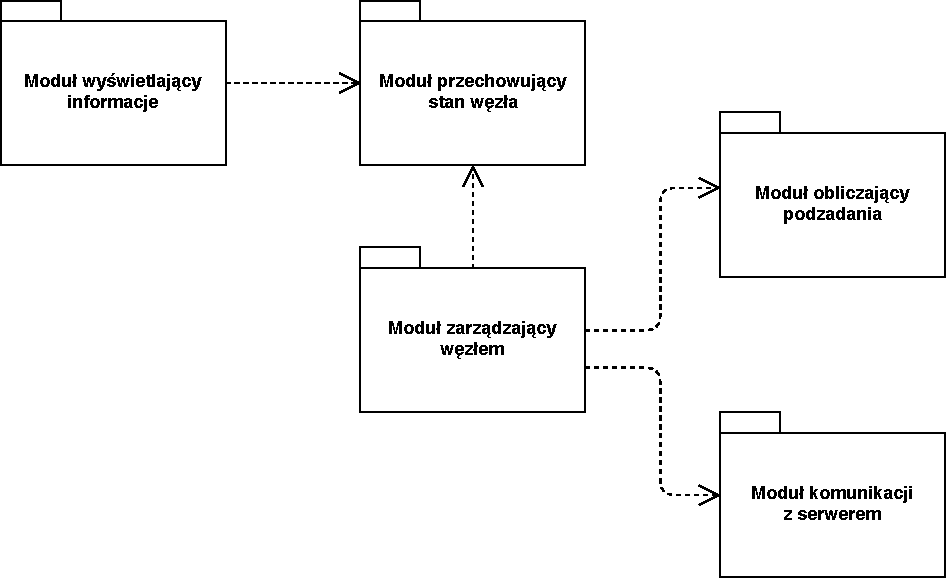
\includegraphics[scale=0.75]{images/moduly-wezla-obliczeniowego.pdf}}
    \caption{Moduły węzłów obliczeniowych.}
    \label{node-model}
\end{figure}


\section{Szczegółowy opis implementacji}

Poniższa sekcja zawiera szczegółowy opis implementacji z podziałem na poszczególne komponenty systemu.


\subsection{Serwer}

Serwer składa się z kontrolerów API działających w oparciu o \textit{ASP.NET Core 2.2}~\cite{aspnet-core}. Obsługują one zapytania dotyczące wszystkich encji na serwerze i wywołują odpowiednie metody serwisów odpowiadających encji. Wywoływane serwisy implementują \textit{EntityResourceService} i pozwalają na umieszczanie dodatkowej logiki pomiędzy kontrolerem, a warstwą dostępu do danych.

Do wywoływania metod z assembly użytkowników (z klasy implementującej interfejs \textit{IProblemPlugin} opisanej w sekcji~\ref{biblioteka-szczegoly}) została wykorzystana klasa \textit{ProblemPluginFacade}. Do utworzenia obiektu tej klasy wykorzystana jest klasa \textit{ProblemPluginFacadeFactory}, której odpowiedzialnością jest wytworzenie takiego obiektu z wejściowego assembly.

W projekcie serwera pojawiają się też klasy odpowiadające modelom w bazie danych. Są to \textit{ProblemPluginInfo}, \textit{DistributedNode}, \textit{Subtask}, \textit{SubtaskInProgress}, \textit{DistributedTask} oraz \textit{DistributedTaskDefinition}.

\textit{DistributedTaskDefinition} jest obiektem odpowiadającym dodanemu problemowi. Jego konkretne instancje z konkretnymi danymi wejściowymi to \textit{DistributedTask}. Każde takie zadanie zostaje rozbite na, z reguły, wiele podzadań (\textit{Subtask}). W momencie, gdy zarejestrowany węzeł obliczeniowy (\textit{DistributedNode}) pyta o nowe zadanie, serwer może przydzielić mu jedno z nieukończonych jeszcze podzadań. Wtedy zostaje utworzona encja \textit{SubtaskInProgress}.



Podczas implementacji serwera zostały zastosowane następujące wzorce projektowe:
\begin{itemize}
    \item Fabryka --- wzorzec fabryki pojawia się w projekcie wielokrotnie. Został on zastosowany aby ułatwić wstrzykiwanie zależności do klas oraz uprościć testowanie projektu.
    \item Fasada --- wzorzec fasady został wykorzystany podczas wywoływania metod z assembly dostarczanych przez użytkowników systemu. Interfejs \textit{IProblemPluginFacade} udostępnia  uproszczoną listę metod możliwych do wykonania na otrzymanym assembly.
    \item Wstrzykiwanie zależności (ang. \textit{dependency injection}) --- wzorzec ten pozwala na ekstrakcję logiki do pobocznych klas oraz wstrzykiwanie ich automatycznie jako parametry konstruktorów. Główną zaletą takiego podejścia jest łatwość testowania, ponieważ wszystkie zależności komponentu są podane w konstruktorze i w testach można wykorzystać zaślepki.
\end{itemize}

Projekt klas serwera znajduje się na rysunkach~\ref{server-class-1},~\ref{server-class-2}.

\begin{figure} \centering{
        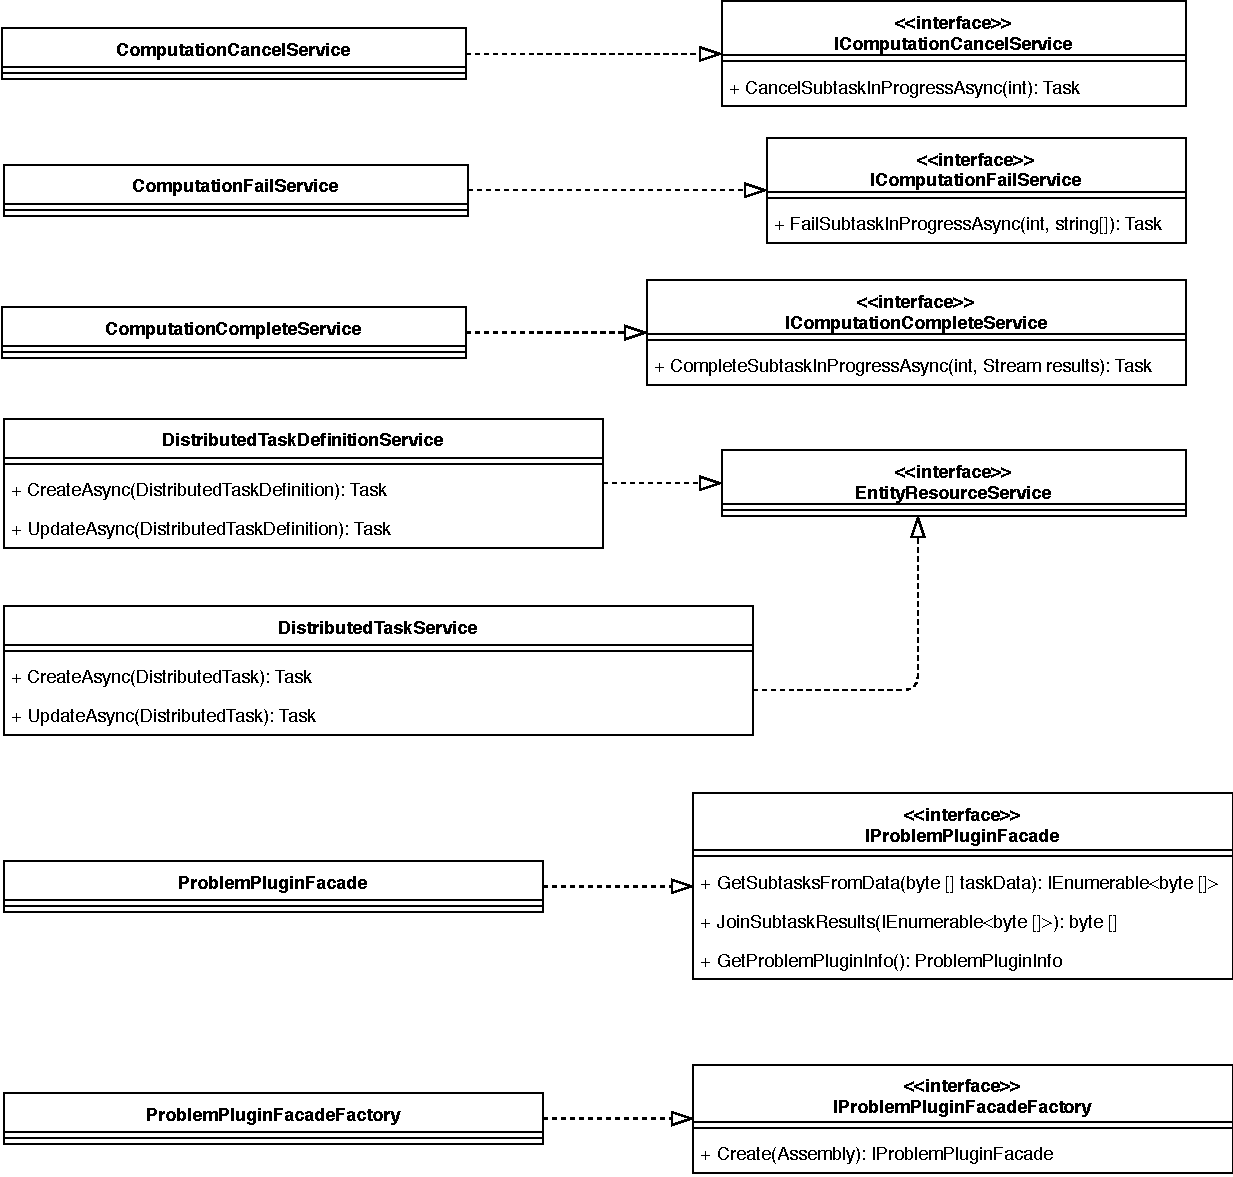
\includegraphics[scale=0.80]{images/server-class-diagram-1.pdf}}
    \caption{Diagram klas serwera.}
    \label{server-class-1}
\end{figure}

\begin{figure} \centering{
        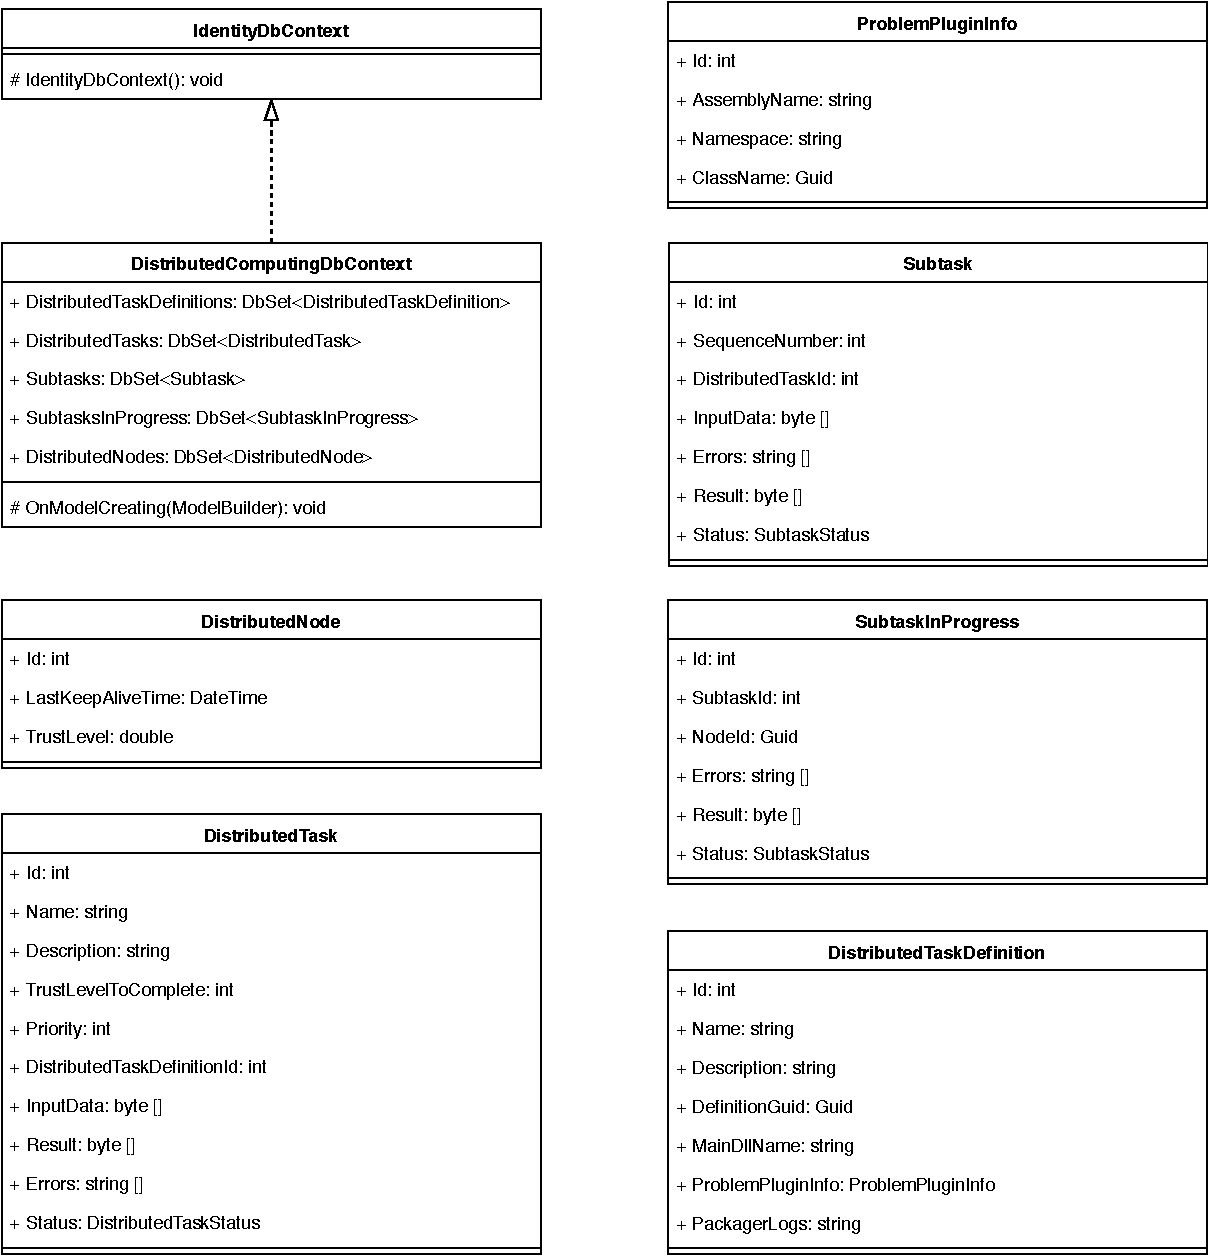
\includegraphics[scale=0.80]{images/server-class-diagram-2.pdf}}
    \caption{Diagram klas serwera dotyczących modeli i bazy danych.}
    \label{server-class-2}
\end{figure}

Schemat bazy danych działającej na serwerze został przedstwiony na rysunku~\ref{database-schema}.

Opis tabel wykorzystanych w bazie danych:
\begin{description}
    \item [DistributedTaskDefinitions] --- zawiera informacje o dodanych definicjach zadań.
    \item [DistributedTasks] --- zawiera informacje o zadaniach utworzonych na podstawie definicji zadania. Dane wejściowe oraz wynik są przechowywane w postaci binarnej.
    \item [Subtasks] --- przechowuje podzadania związane z instancjami zadań.
    \item [SubtasksInProgress] --- przechowuje uruchomione obliczenia podzadań. Podzadanie może być uruchomione wielokrotnie, zależnie od zadanego poziomu zaufania dla całego zadania.
    \item [DistributedNodes] --- przechowuje informacje o węzłach obliczeniowych.
    \item [AspNetUsers] --- tabela zawiera informacje o użytkownikach, którzy mają dostęp do systemu. 
\end{description}

\begin{figure} \centering{
        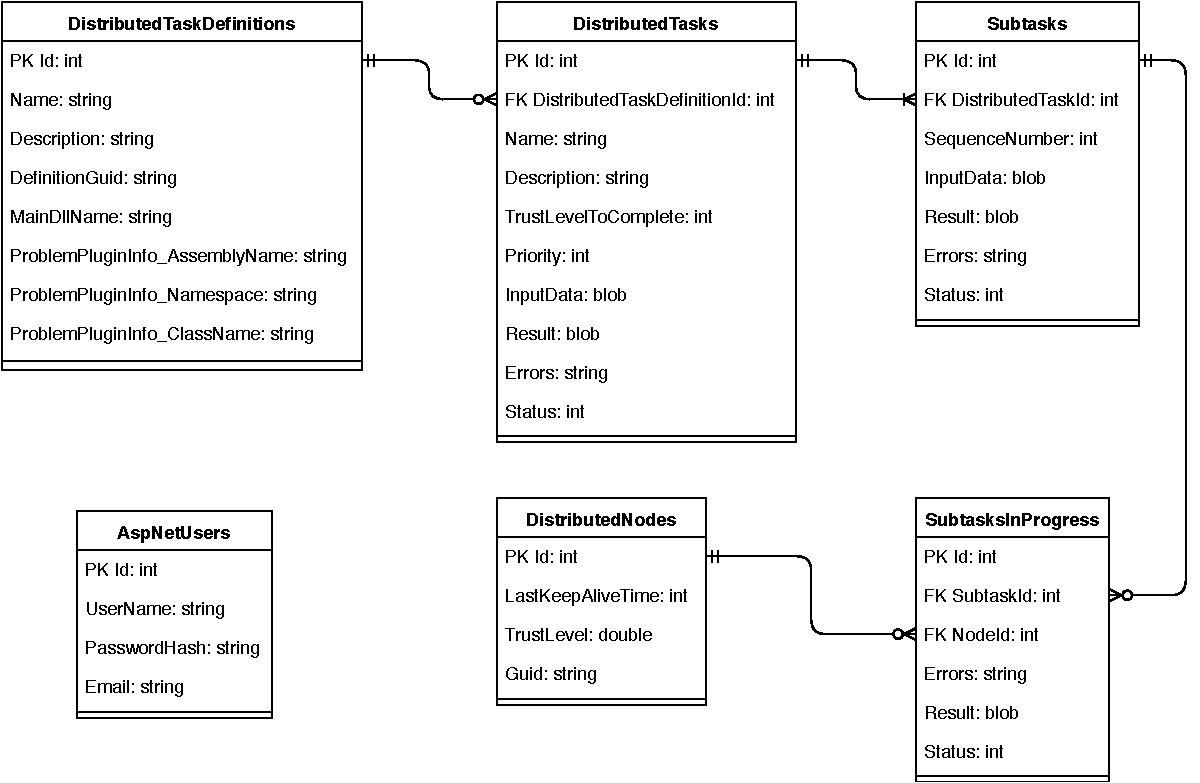
\includegraphics[scale=0.75,page=1]{images/database-schema.pdf}}
    \caption{Schemat bazy danych działającej na serwerze.}
    \label{database-schema}
\end{figure}


Rysunek~\ref{task-state-diagram} przedstawia diagram stanów dla zadań.

Zadanie (\texttt{DistributedTask}) początkowo znajduje się w stanie \textit{W trakcie wykonania}. W miarę wykonywania jego podzadań (\texttt{Subtask}) zadanie albo będzie pozostawało w stanie \textit{W trakcie wykonania} jeżeli będą podzadania, które nie zostały jeszcze wykonane, albo przejdzie do stanu \textit{Wykonane}, jeżeli nie będzie już podzadań do wykonania. Wtedy serwer scali wyniki podzadań w wynik zadania i zapisze je w bazie danych. W przypadku gdy którekolwiek z podzadań zakończy się błędem, całe zadanie zostaje oznaczone jako \textit{Zakończone błędem}.


\begin{figure} \centering{
        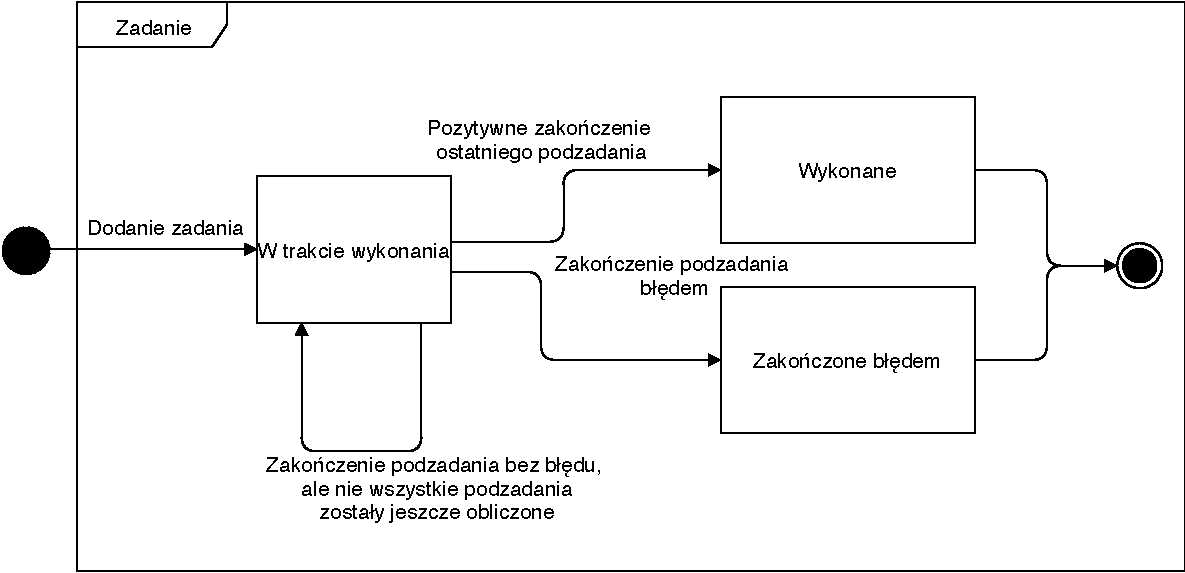
\includegraphics[scale=0.75]{images/task-state-diagram.pdf}}
    \caption{Diagram stanów dla zadania.}
    \label{task-state-diagram}
\end{figure}

Rysunek~\ref{subtask-state-diagram} przedstawia diagram stanów dla podzadań.

Podzadanie po utworzeniu oczekuje na wykonanie przez pewne węzły. Gdy zadanie zostaje przydzielone pewnemu węzłowi, przechodzi one do stanu \textit{W trakcie obliczeń}. Z uwagi na poziomy zaufania węzłów (opisane w sekcji~\ref{poziom-zaufania-wezlow}) podzadanie może zostać wykonane przez kilka węzłów. Do zamodelowania obliczania danego podzadania przez konkretny węzeł służy klasa \texttt{SubtaskInProgress}. W trakcie obliczania wyniku przez węzeł może pojawić się błąd. W takim przypadku w zależności od tego czy limit prób został już wyczerpany czy nie, podzadanie odpowiednio przechodzi do stanu \textit{Zakończone błędem} lub pozostaje w stanie \textit{W trakcie obliczeń}. Jeżeli obliczenie przebiegnie bezbłędnie, zadanie przechodzi do stanu \textit{Wykonane}. Wynik podzadania zostanie zapisany w bazie danych.

\begin{figure} \centering{
        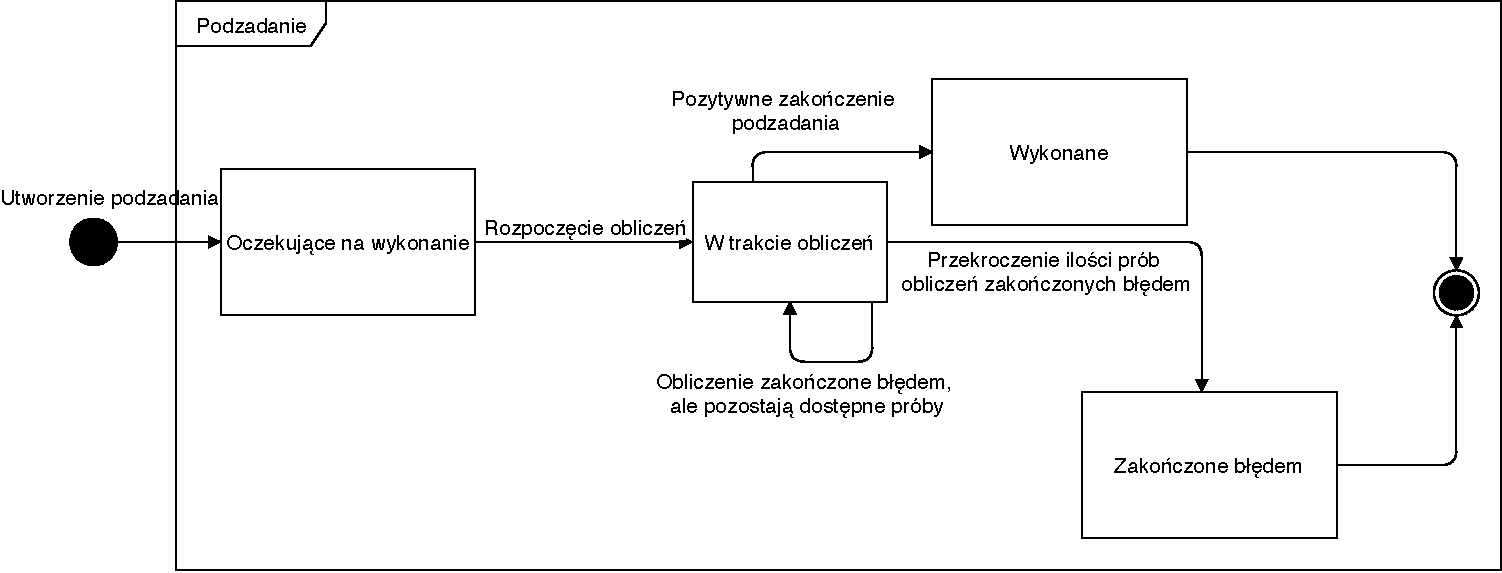
\includegraphics[scale=0.65]{images/subtask-state-diagram.pdf}}
    \caption{Diagram stanów dla podzadania.}
    \label{subtask-state-diagram}
\end{figure}


Na rysunku~\ref{task-definition-sequence-diagram} został przedstawiony diagram sekwencji dla dodawania nowej definicji zadania z wykorzystaniem API udostępnianego przez serwer.

Na początku użytkownik przesyła assembly, w którym istnieje klasa implementująca wspomniany już interfejs \textit{IProblemPlugin}. Dodatkowo użytkownik powinien załączyć pozostałe biblioteki wykorzystywane w projekcie. Po przesłaniu tych plików na serwer zostają one zapisane na dysku, po czym assembly zawierające implementację interfejsu \textit{IProblemPlugin} zostaje wczytane i przeanalizowane pod kątem poprawności. Jeżeli assembly jest poprawne, informacje o nowej definicji zadania zostają dodane do bazy danych, a informacja o sukcesie zostaje zwrócona użytkownikowi.

\begin{figure} \centering{
        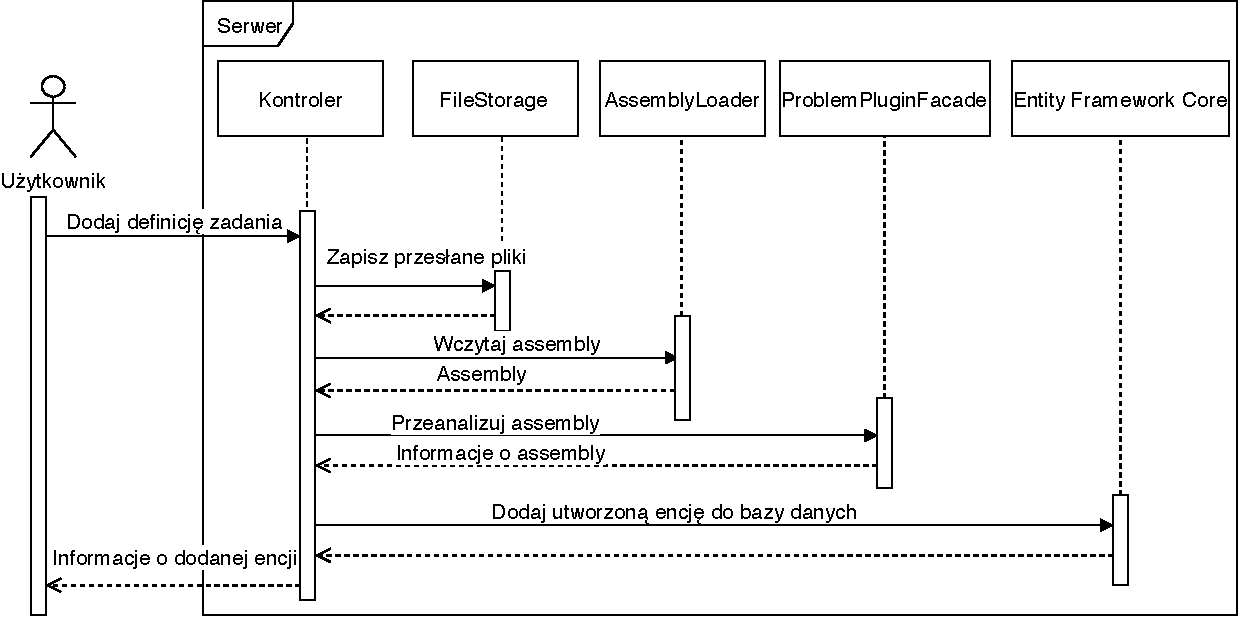
\includegraphics[scale=0.75]{images/sequence-diagram.pdf}}
    \caption{Diagram sekwencji dla dodawania nowej definicji zadania.}
    \label{task-definition-sequence-diagram}
\end{figure}

\subsubsection{Wykorzystane technologie}
Serwer został zaimplementowany w języku C\# wykorzystując technologię \textit{.NET Core 2.2}~\cite{dotnet-core} oraz \textit{ASP.NET Core}~\cite{aspnet-core}. Jako baza danych wykorzystana została baza \textit{PostgreSQL}~\cite{postgresql}. Do komunikacji z bazą danych wykorzystano \textit{Entity Framework Core}~\cite{ef-core}.

Standardem formatu przesyłu danych do API oraz odbioru odpowiedzi z API jest standard \textit{JSON API}~\cite{jsonapi}. W celu zgodności z tym standardem wykorzystano bibliotekę \textit{JSON API .NET Core}~\cite{jsonapi-dotnet-core}. Użyta biblioteka udostępnia generyczne kontrolery, które implementują wszystkie akcje wymagane przez standard \textit{JSON API} po podaniu modelu obsługiwanego przez kontroler. Wykorzystanie tak utworzonych kontrolerów pozwoliło na zaoszczędzenie czasu podczas tworzenia API.

Do przekształcenia assembly użytkownika do wersji możliwej do uruchomienia w \textit{WebAssembly} wykorzystano \textit{Software Development Kit} (SDK) \textit{mono-wasm}~\cite{mono-wasm}.

Testy jednostkowe zostały napisane z wykorzystaniem bibliotek \textit{NUnit} oraz \textit{Moq}.

\subsection{Biblioteka do implementacji algorytmów rozproszonych}
\label{biblioteka-szczegoly}

Projekt klas biblioteki ułatwiającej tworzenie algorytmów rozproszonych znajduje się na rysunku~\ref{library-class}.

Interfejs \textit{IProblemPlugin} wymaga implementacji:
\begin{itemize}
    \item Metody \textit{DivideTask} --- przyjmuje ona zadanie wejściowe i dzieli je na podzadania. Metoda jest uruchamiana na serwerze.
    \item Metody \textit{Compute} --- przyjmuje ona dane wejściowe dla podzadania i wykonuje na ich podstawie obliczenia, zwracając ostatecznie wynik. Metoda jest uruchamiana na węzłach obliczeniowych.
    \item Metody \textit{JoinSubtaskResults} --- przyjmuje ona kolekcję składającą się z wyników obliczonych podzadań i zwraca wyznaczony wynik końcowy. Metoda ta uruchamiana jest na serwerze.
    \item Czterech obiektów implementujących interfejs \textit{IDataFormatter} pozwalających na serializację oraz deserializację danych wejściowych oraz wyników zadania i podzadania (klasy \textit{TTask, TTaskResult, TSubtask, TSubtaskResult}).
    
    Dane serializowane i deserializowane są w następujący sposób. Po przesłaniu pliku zawierającego zserializowane zadanie \textit{TTask}, zadanie to zostaje zdeserializowane na serwerze i za pomocą metody \textit{DivideTask} podzielone na podzadania \textit{TSubtask}, po czym podzadania te zostają zserializowane i zapisane w bazie danych.
    
    Następnie po przydzieleniu podzadania do konkretnego węzła i pobraniu tego zserializowanego podzadania, węzeł deserializuje to podzadanie, po czym oblicza jego wynik metodą \textit{Compute}. Wynik \textit{TSubtaskResult} jest serializowany i przesyłany na serwer, który umieszcza wynik w bazie danych.
    
    W momencie, gdy ostatnie podzadanie zostaje ukończone, wyniki wszystkich podzadań \textit{TSubtaskResult} są pobierane przez serwer z bazy danych, następnie uruchamiana jest metoda \textit{JoinSubtaskResults}, po czym wynik zadania \textit{TTaskResult} jest zapisywany przez serwer w bazie danych.
\end{itemize}

\begin{figure} \centering{
        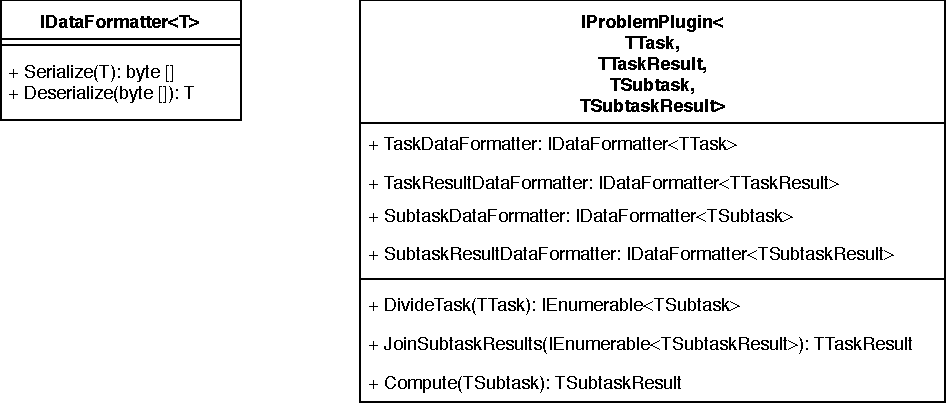
\includegraphics{images/library-class-diagram.pdf}}
    \caption{Diagram klas biblioteki wspomagającej tworzenie algorytmów rozproszonych.}
    \label{library-class}
\end{figure}

\subsubsection{Wykorzystane technologie}
Biblioteka do implementacji algorytmów rozproszonych została zaimplementowana w języku C\# w technologii \textit{.NET Standard 2.0}~\cite{dotnet-standard}.

\subsection{Węzły obliczeniowe}

Węzły obliczeniowe składają się z panelu sterowania węzłem, kontrolera działającego po stronie przeglądarki (napisanego w języku \textit{Typescript}) oraz wątków wykonujących faktyczne obliczenia.

Diagram stanów węzła obliczeniowego został przedstawiony na rysunku~\ref{node-state}.

Węzeł początkowo jest nieaktywny. Po naciśnięciu przycisku zostaje on aktywny -- rejestruje się na serwerze oraz próbuje otrzymać nowe zadania. W momencie otrzymania nowego zadania pobiera on kod oraz dane wejściowe potrzebne do jego obliczenia. Jeżeli podczas obliczeń wystąpił błąd, zostaje o tym powiadomiony serwer, a węzeł ponownie pyta o nowe zadania.

W momencie, gdy obliczenie zostało zakończone sukcesem, wynik zostaje zwrócony do serwera, a węzeł pyta o nowe zadania.

W dowolnym momencie osoba posiadająca dostęp do interfejsu węzła (określana dalej jako właściciel węzła) może zdecydować o zakończeniu obliczeń. Wtedy węzeł wraca do stanu \textit{Nieaktywny}. W tej sytuacji węzeł powiadamia serwer, że wszystkie zadania obliczane przez niego w tym momencie powinny być uznane jako anulowane.

Ponadto, właściciel węzła może skonfigurować ile zadań może być jednocześnie obliczanych w różnych wątkach na tym węźle.

\begin{figure} \centering{
        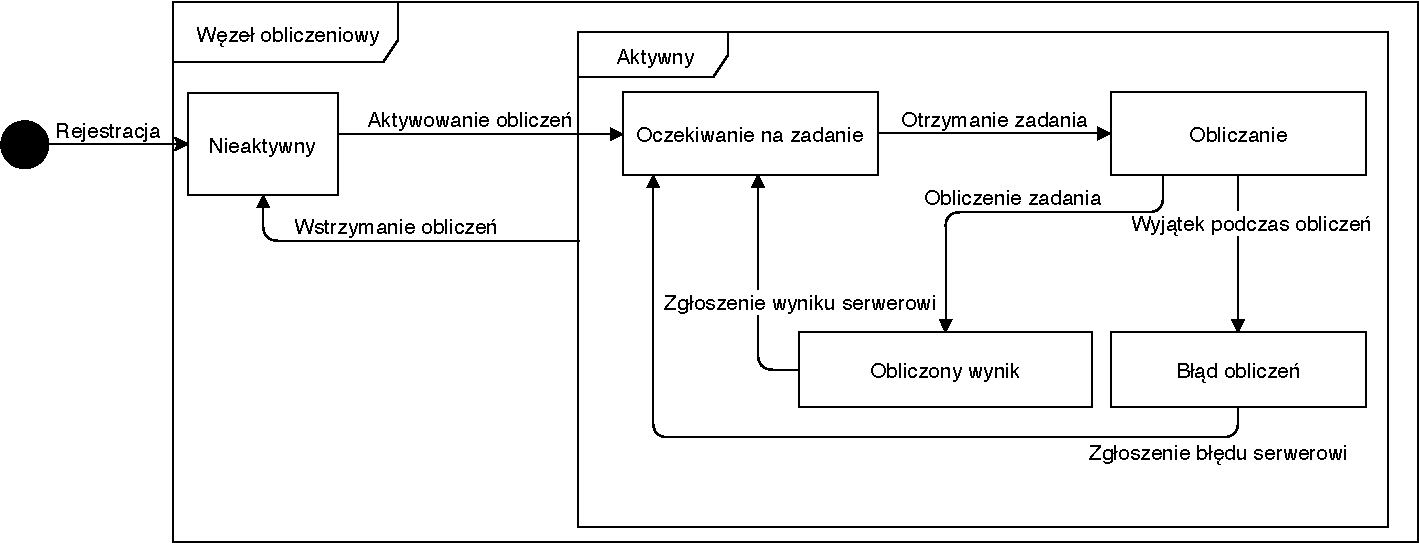
\includegraphics[scale=0.8]{images/node-state-diagram.pdf}}
    \caption{Diagram stanów węzła obliczeniowego.}
    \label{node-state}
\end{figure}

\subsubsection{Wykorzystane technologie}
Węzły obliczeniowe zostały zaimplementowane w języku \textit{Typescript}~\cite{typescript} wykorzystując framework \textit{React}~\cite{react} we wzorcu MVVM (\textit{Model, View, ViewModel})~\cite{mvvm}.

Wzorzec ten zakłada, że dane (\textit{Model}) i ich prezentacja (\textit{View}) są od siebie oddzielone, a warstwą komunikującą jest \textit{ViewModel}, który jest również oddzielnym komponentem.

Wykorzystanie wzorca MVVM zapewnia niezależność logiki od interfejsu użytkownika oraz pozwala na łatwe przeprowadzanie testów jednostkowych.

Celem uzyskania generowania kodu HTML po stronie serwera (z angielskiego \textit{Server Side Rendering} -- SSR) wykorzystano bibliotekę \textit{next.js}~\cite{next.js}.

Wykorzystano również komponenty interfejsu użytkownika z biblioteki \textit{evergreen}~\cite{evergreen}.

Uprzednio skompilowany kod wykonujący obliczenia rozproszone jest uruchamiany w środowisku \textit{WebAssembly}.

Testy jednostkowe zostały napisane z wykorzystaniem biblioteki \textit{jest}~\cite{jest}. Podczas testów end-to-end został wykorzystany framework \textit{Cypress}~\cite{cypress}.

\subsection{Panel administracyjny}

Panel administracyjny umożliwia uwierzytelnienie, a po jego dokonaniu zarządzanie systemem. Obsługiwany jest poprzez aplikację internetową działającą w przeglądarce.

Podczas implementacji panelu administracyjnego wielokrotnie wykorzystany został wzorzec \textit{dekorator}. Stosowaniu dekoratorów pozwaliło na rozszerzenie możliwości oferowanych przez uniwersalne komponenty interfejsu i dostosowywanie ich do poszczególnych widoków w taki sposób, żeby nie powielać kodu.


\subsubsection{Wykorzystane technologie}
Panel administracyjny, podobnie do węzłów obliczeniowych, został zaimplementowany w języku \textit{Typescript}~\cite{typescript} z użyciem frameworka \textit{React}~\cite{react} oraz \textit{next.js}~\cite{next.js} zapewniającego generowanie kodu HTML po stronie serwera. Wykorzystany został wzorzec MVVM~\cite{mvvm}.

Do elementów interfejsu użytkownika poza wspomniano poprzednio biblioteką \textit{evergreen}~\cite{evergreen} wykorzsystano bibliotekę \textit{react-table}~\cite{react-table} do wyświetlania tabel oraz bibliotekę \textit{formik}~\cite{formik} do wyświetlania i zarządzania formularzami.

Aby ułatwić pracę ze standardem \textit{JSON API} wykorzystano bibliotekę \textit{kitsu}~\cite{kitsu}.

Testy jednostkowe zostały napisane z wykorzystaniem biblioteki \textit{jest}~\cite{jest}.


\section{Zabezpieczenia}

Poniższa sekcja opisuje zabezpieczenia wykorzystywane w projekcie.

\subsection{Uwierzytelnianie} 

Dostęp do panelu administracyjnego wymagania uwierzytelnienia, czyli podania loginu oraz hasła administratora. Jeżeli dane te zgadzają się z danymi zapisanymi w bazie danych, użytkownik dostaje dostęp do panelu.

W przeciwnym wypadku użytkownik nie będzie miał możliwości pobrania żadnych danych ani wykonania jakichkolwiek operacji na encjach.

Jedyne operacje, które są dostępne publicznie, to zarejestrowanie urządzenia jako węzeł obliczeniowy, żądanie przydzielenia nowego zadania, zwrócenie wyniku lub informacji o błędzie. Są to operacje wymagane do prawidłowego funkcjonowania węzłów obliczeniowych. Wszystkie inne operacje są dostępne dopiero po uwierzytelnieniu.

\subsection{Ograniczenia przy zwracaniu wyników}

Każdy węzeł posiada unikatowy identyfikator przyznany mu w momencie rejestracji. Podczas anulowania zadania, zwracania wyników obliczeń lub informacji o błędzie serwer sprawdzi czy identyfikator węzła wysyłającego żądanie zgadza się z identifykatorem węzła przypisanego do aktualizowanego zadania. Jeżeli nie, serwer nie zmieni statusu zadania.

\subsection{Poziom zaufania węzłów}
\label{poziom-zaufania-wezlow}

Może zdarzyć się taka sytaucja, że jako węzły obliczeniowe dołączą urządzenia, które celowo będą wysyłały niepoprawne wyniki obliczeń.

Aby nie zakłóciło to natychmiast pracy systemu z każdym węzłem obliczeniowym jest powiązany jego \textit{poziom zaufania}. Tworząc nowe zadanie z konkretnymi danymi wejściowymi administrator ustawi wymagany poziom zaufania do zakończenia obliczeń podzadań.

Każde z podzadań utworzonych na podstawie zadania będzie uznawane za zakończone, gdy suma poziomów zaufania węzłów, które zwróciły wyniki przekroczy wymagany poziom zaufania zadania.

Wynikiem każdego z podzadań będzie wynik, dla którego suma poziomów zaufania węzłów, które go zwróciły, była maksymalna.

Dla przykładu przyjmijmy, że mamy w systemie zadanie z zdefiniowanym wymaganym poziomie zaufania 5. W tabeli~\ref{trust-level-example} zostały przedstawione węzły wykonujące jedno z podzadań tego zadania wraz z wynikamchk i oraz ich poziomem zaufania.

\begin{table}[ht]
    \centering
    \caption{Przykładowe węzły obliczeniowe wraz z ich poziomami zaufania oraz wynikami, które zwróciły}
    \label{trust-level-example}
    \begin{tabular}{|l|l|l|}
        \hline
        Węzeł & Wynik & Poziom zaufania \\ \hline
        A     & 1     & 2.5             \\ \hline
        B     & 1     & 1               \\ \hline
        C     & 5     & 2               \\ \hline
    \end{tabular}
\end{table}

Podzadanie zostanie zakończone, ponieważ suma poziomów zaufania jest większa od wymaganego poziomu zaufania:

\[2.5 + 1 + 2 = 5,5 > 5\]

Ponadto, wynikiem zadania będzie 1, ponieważ wynik ten został zwrócony przez węzły o sumarycznym poziomie zaufania 3.5, podczas gdy wynik 5 został zwrócony przez węzły o sumarycznym poziomie zaufania 2.

\chapter{Opis aplikacji}
    Poniższy rozdział opisuje przygotowane rozwiązanie. Na potrzeby tego rozdziału zostały utworzone: lista wykorzystywanych bibliotek wraz z ich licencjami, instrukcje przydatne podczas pracy z opisywanym systemem oraz lista testów akceptacyjnych wraz z ich rezultatami.
    
    \section{Wykorzystane biblioteki}
         W tej sekcji zostaną przedstawione wykorzystane biblioteki z podziałem na część serwera aplikacyjnego i część udostępniającą interfejs użytkownika.
        
        \subsection{Biblioteki serwera aplikacyjnego}
        Tabela \ref{biblioteki-serwer} zawiera biblioteki użyte w serwerze aplikacyjnym wraz z ich licencjami.
        
        \begin{center}
            \begin{longtable}{| p{.10\textwidth} | p{.20\textwidth} | p{.40\textwidth} | p{.15\textwidth} |}
                \caption{Wykorzystane biblioteki w serwerze aplikacyjnym wraz z ich licencjami}
                \label{biblioteki-serwer} \\
                \hline
                nr. & Nazwa i wersja & Opis & Licencja \\ \hline
                \endfirsthead
                \multicolumn{4}{c}{\tablename\ \thetable\ -- \textit{Kontynuowane z poprzedniej strony}} \\
                \hline
                nr. & Nazwa i wersja & Opis & Licencja \\ \hline
                \endhead
                
                1 & ASP.NET Core v2.2.0 & Framework do tworzenia serwerów API. & Apache 2.0 \\ \hline
                2 & JSON API .NET Core v2.4.0 & Biblioteka pozwalająca na tworzenie kontrolerów API zgodnych ze standardem JSON API. & MIT \\ \hline
                3 & Entity Framework Core v2.2.0 & Biblioteka pozwalająca na łatwą komunikację z bazą danych z poziomu kodu. & Apache 2.0 \\ \hline
                4 & Npgsql EntityFrameworkCore PostrgreSQL v2.2.0 & Biblioteka pozwalająca na komunikację z bazą danych PostgreSQL. & PostgreSQL \cite{licencja-postgresql} \\ \hline
                5 & Mono v5.16.0 & Implementacja .NET Framework działająca w systemie UNIX. & Własna licencja Mono \cite{licencja-mono} \\ \hline
                6 & mono-wasm v5.16.0 & Interpreter języka C\# działający w technologii WebAssembly. & Własna licencja Mono \cite{licencja-mono} \\ \hline
                7 & NUnit 3.11.0 & Biblioteka do tworzenia i uruchamiania testów jednostkowych. & NUnit License \cite{licencja-nunit} \\ \hline
                8 & Moq v4.10.1 & Biblioteka pozwalająca na tworzenie zaślepek podczas testów jednostkowych. & BSD-3-Clause \\ \hline
            \end{longtable}
        \end{center}
        
        \subsection{Biblioteki serwera udostępniającego interfejs użytkownika}
        Tabela \ref{biblioteki-frontend} zawiera biblioteki użyte w serwerze budującym i wyświetlającym interfejs użytkownika wraz z ich licencjami.
        
        \begin{center}
            \begin{longtable}{| p{.10\textwidth} | p{.20\textwidth} | p{.40\textwidth} | p{.15\textwidth} |}
                \caption{Wykorzystane biblioteki w serwerze interfejsu użytkownika wraz z ich licencjami}
                \label{biblioteki-frontend} \\
                \hline
                nr. & Nazwa i wersja & Opis & Licencja \\ \hline
                \endfirsthead
                \multicolumn{4}{c}{\tablename\ \thetable\ -- \textit{Kontynuowane z poprzedniej strony}} \\
                \hline
                nr. & Nazwa i wersja & Opis & Licencja \\ \hline
                \endhead
                
                1 & date-fns v1.30.1 & Biblioteka do łatwego zarządzania datami & MIT \\ \hline
                2 & evergreen-ui v4.0.2 & Biblioteka z komponentami interfejsu użytkownika & MIT \\ \hline
                3 & express v4.16.4 & Biblioteka pozwalająca na stworzenie serwera HTTP w Node.js & MIT \\ \hline
                4 & formik v1.3.1 & Biblioteka do zarządzania formularzami w aplikacji & MIT \\ \hline
                5 & immutable v4.0.0-rc.11 & Biblioteka dostarczająca niezmienne struktury danych & MIT \\ \hline
                6 & kitsu v6.4.0 & Biblioteka do komunikacji z JSON API & MIT \\ \hline
                7 & next v7.0.2 & Framework do budowania aplikacji przeglądarkowych w React umożliwiający Server-Side Rendering & MIT \\ \hline
                8 & normalize.css v8.0.1 & Biblioteka od normalizacji stylowania komponentów w przeglądarce & MIT \\ \hline
                9 & path-to-regexp v2.4.0 & Biblioteka pozwalająca na sprawdzenie czy URL pasuje do danej ścieżki na stronie & MIT \\ \hline
                10 & ramda v0.25.0 & Biblioteka udostępniająca wiele pomocniczych funkcji & MIT \\ \hline
                11 & React v16.5.2 & Framework do wyświetlania interfejsów użytkownika & MIT \\ \hline
                12 & React-table v6.8.6 & Biblioteka udostępniająca komponent tabeli & MIT \\ \hline
                13 & yup v0.26.6 & Biblioteka udostępniająca narzędzia do budowania walidatorów danych & MIT \\ \hline
                14 & jest v23.6.0 & Biblioteka umożliwiająca tworzenie i uruchamianie testów jednostkowych & MIT \\ \hline
            \end{longtable}
        \end{center}
    
    \section{Platforma docelowa}
        Do instalacji i uruchomienia projektu wymagany jest system o następujących parametrach:
        
        \begin{itemize}
            \item System operacyjny Arch Linux 
            \item Minimalnie 2 GB pamięci RAM
            \item Minimalnie 10 GB pamięci dyskowej
        \end{itemize}
        
        Do uruchomienia systemu potrzebne będą następujące programy:
        
        \begin{itemize}
            \item Docker (w wersji minimalnie 18.09.0)
            \item Docker-compose (w wersji minimalnie 1.23.2)
        \end{itemize}
    
        Instrukcja instalacji wymienionych aplikacji dostępna jest w sekcji \ref{installation-instruction}.
    
    \section{Instrukcje}
        Poniższy rozdział zawiera instrukcje dotyczące instalacji, wdrożenia, uruchomienia, użycia oraz utrzymania systemu.
    
    \subsection{Instrukcja instalacji}
        \label{installation-instruction}
        W celu instalacji wymaganych zależności należy zainstalować pakiety \textit{docker} oraz \textit{docker-compose}, a następnie uruchomić serwis \textit{docker} komendą:

        \begin{verbatim}
    # systemctl start docker
        \end{verbatim}

        W celu weryfikacji działania serwisu \textit{docker} należy wywołać komendę:
        \begin{verbatim}
    # docker ps
        \end{verbatim}

        Jeśli po uruchomieniu powyższej komendy pojawi się tabelka, to znaczy, że instalacja się powiodła.

    \subsection{Instrukcja wdrożenia}
    
        Jeśli projekt jest uruchamiany na serwerze, który nie posiada ograniczeń w dostępie do sieci, to można przejść do podpunktu \ref{start-system}. W przeciwnym wypadku należy zbudować obrazy \textit{Docker} na maszynie z dostępem do sieci, a następnie skopiować przygotowane obrazy na maszynę docelową, na której system ma być uruchomiony.
        
        Zakładamy, że katalog zawierający kod źródłowy projektu nazwany jest \texttt{distributed-computing-webworker}. Jeżeli będzie nazwany w inny sposób, poniższe komendy powinny zostać zmodyfikowane, zamieniając \texttt{distributed-computing-webworker} w nazwach obrazów na nazwę katalogu, w którym znajduje się kod źródłowy projektu. 
        W celu zbudowania obrazów \textit{Docker} należy wywołać następujące komendy na maszynie budującej:

        \begin{verbatim}
    # docker-compose -f docker-compose.yml -f docker-compose.prod.yml \
        up --build --no-start
    # docker save distributed-computing-webworker_backend \
        distributed-computing-webworker_frontend postgres \
        nginx | gzip > docker_images.tar.gz    
        \end{verbatim}

        Następnym krokiem jest skopiowanie wyeksportowanych obrazów oraz plików \textit{docker-compose.yml}, \textit{docker-compose.prod.yml} na maszynę docelową. Można to wykonać na przykład wykorzystując narzędzie \textit{scp}.
        Po zakończeniu kopiowania należy zaimportować skopiowane obrazy do \textit{Docker} uruchomionego na maszynie docelowej wywołując na niej następującą komendę:

        \begin{verbatim}
    # gunzip -c ~/docker_images.tar.gz | docker load
        \end{verbatim}

    \subsection{Instrukcja uruchomienia}
        \label{start-system}
        Aby uruchomić projekt należy z katalogu zawierającego pliki \textit{docker-compose.yml}, \textit{docker-compose.prod.yml} wywołać komendę:

        \begin{verbatim}
    # docker-compose -f docker-compose.yml -f docker-compose.prod.yml up -d
        \end{verbatim}

        Jeśli w systemie nie znajdują się zbudowane obrazy \textit{Docker}, to podczas trwania tej komendy zostaną one zbudowane.
        Po zakończeniu wykonywania komendy działanie systemu można zweryfikować przez próbę wejścia na adres \url{http://[adres_serwera]}. Jeśli uruchomienie systemu się powiodło, to powinna zostać wyświetlona strona zawierająca informacje o projekcie.

    \subsection{Instrukcja utrzymania}

        Poniższa sekcja zawiera informacje dotyczące zarządzania stanem całego systemu oraz opis tworzenia kopii zapasowej i przywracania jej.

        \subsubsection{Usunięcie systemu}

            Aby skasować system wraz z wszelkimi danymi zawartymi w nim należy użyć komendy:

            \begin{verbatim}
   # docker-compose -f docker-compose.yml -f docker-compose.prod.yml down
            \end{verbatim}


        \subsubsection{Zatrzymanie systemu}

            Aby zatrzymać system zachowując dane należy użyć komendy:
            
            \begin{verbatim}
   # docker-compose -f docker-compose.yml -f docker-compose.prod.yml stop
            \end{verbatim}

            Ponowne uruchomienie systemu należy wykonać zgodnie z punktem \ref{start-system}.

        \subsubsection{Tworzenie kopii zapasowej}

            Aby utworzyć kopię zapasową należy uruchomić skrypt \textit{backup.sh} znajdujący się w katalogu \textit{scripts} umieszczonym w głównym folderze projektu. 
            Kopia bazy danych oraz definicji zadań zostanie zapisana w pliku \textit{backup\_data.tar.gz}
            
        \subsubsection{Przywracanie kopii zapasowej}

            Aby przywrócić kopię zapasową należy uruchomić skrypt \textit{restore.sh} podając jako argument nazwę archiwum zawierającego kopię zapasową, stworzonego za pomocą skryptu z poprzedniego kroku. Skrypt \textit{restore.sh} znajduje się w katalogu \textit{scripts} w głównym folderze projektu.
            
    \subsection{Instrukcja użycia}
        W poniższej sekcji przedstawiono instrukcję użycia produktu z podziałem na etap logowania, dodawania definicji zadania, dodawania zadania, obliczania zadania oraz pobierania wyników.
        
        \subsubsection{Logowanie}
        
        Po uruchomieniu systemu interfejs użytkownika dostępny jest pod adresem \url{http://[adres_serwera]}. Dostęp do wykonywania obliczeń dostępny jest dla wszystkich użytkowników, a panel administracyjny wymaga zalogowania.
        Domyślne dane do logowania do panelu administracyjnego:

        \begin{verbatim}
    login: admin
    hasło: D1stributed$
        \end{verbatim}


        Po pierwszym zalogowaniu należy zmienić domyślne hasło. Opcja zmiany hasła jest dostępna z poziomu paska bocznego.
        
        \subsubsection{Dodanie definicji zadania}
        \label{distributed-task-definition-add-guide}
        
        Aby dodać nową definicję zadania należy przejść do zakładki \texttt{Distributed Task Definitions}. 
        Po przejściu do zakładki z definicjami zadań zostanie wyświetlona tabela zawierająca zadania dodane już do systemu. 
        W prawym górnym rogu znajduje się ikona plusa na zielonym tle, po kliknięciu w nią nastąpi przekierowanie do formularza dodawania nowej definicji zadania.
        Aby dodać nową definicję zadania należy wypełnić wyświetlony formularz.
        
        W polu \textit{MainDLL} należy umieścić bibliotekę implementującą interfejs \textit{IProblemPlugin} z biblioteki \textit{DistributedComputingLibrary}.
        W polu \textit{AdditionalDlls} powinny zostać wybrane wszystkie pozostałe biblioteki znajdujące się w folderze wynikowym zbudowanej definicji zadania.
        Po wypełnieniu wszystkich pól należy wysłać formularz klikając przycisk \texttt{Submit}.
        Po dodaniu nowej definicji zadania następuje przekierowanie do strony wyświetlającej szczegóły dodanego zadania. 
        
        Przykładowe zadania dostępne są w folderze \textit{example-problems} znajdującym się w głównym katalogu projektu.
        
        
        \subsubsection{Dodanie nowego zadania}
        \label{distributed-task-add-guide}
        
        Aby dodać nowe zadanie należy przejść do zakładki \texttt{Distributed Task Definitions}, a następnie kliknąć w przycisk z napisem \texttt{See details} przy wybranej definicji zadania.
        Z tej strony możemy zlecić obliczenia nowych danych wejściowych.
        W tym celu należy kliknąć na ikonę plusa na zielonym tle znajdującego się nad tabelą z zadaniami.
        W celu zlecenia wykonania zadania należy wypełnić widoczny formularz.
        
        Pole \textit{Priority} określa priorytet zadania, im jest wyższy, tym szybciej zostanie ono przekazane do wykonania.
        Pole \textit{Trust level to complete} określa wymaganą sumę poziomów zaufania węzłów obliczeniowych wykonujących każde z podzadań, aby móc je zakończyć. 
        W polu \textit{Task input} należy umieścić plik zawierający dane wejściowe.
        Po wypełnieniu wszystkich pól należy wysłać formularz klikając w przycisk \texttt{Submit}. Po kliknięciu nastąpi przekierowanie do detali utworzonego zadania. 
        W skład detali wchodzą informacje o utworzonym zadaniu oraz status poszczególnych podzadań. W górnej części widocznej strony znajdują się również przyciski pozwalające na zarządzanie zadaniem oraz pobranie danych wejściowych.
        
        \subsubsection{Rozpoczęcie obliczeń}
        
        Aby obliczenia się rozpoczęły do systemu musi dołączyć co najmniej jeden węzeł obliczeniowy. Aby urządzenie chcące zostać węzłem obliczeniowym dołączyło do systemu, musi ono wejść do zakładki \texttt{Worker} dostępnej w pasku bocznym, a następnie kliknąć na przycisk \texttt{Start the worker}.
        Po kliknięciu w przycisk urządzenie zaczynie odpytywać o nowe zadania.
        Węzły sieciowe mogą w każdym momencie przerwać obliczenia przez kliknięcie w przycisk \texttt{Stop the worker} oraz dowolnie konfigurować ilość udostępnianych wątków. 
        
        
        Stan węzła obliczeniowego jest dostępny w sekcji \textit{Worker information}, a status użyczonych wątków jest udostępniony do wglądu w tabeli \textit{Individual thread statuses}. W momencie, gdy stan węzła zawiera informację o braku dostępnych zadań do obliczenia wiemy, że nasze zadanie zostało wykonane.
        
        
        \subsubsection{Sprawdzenie wyników}
        
        Aby sprawdzić rezultat zleconego zadania należy wybrać opcję \texttt{Distributed Tasks} w panelu bocznym.
        Strona ta zawiera zadania znajdujące się w systemie.
        Aby sprawdzić wynik dodanego wcześniej zadania należy kliknąć w przycisk \texttt{See details} w wierszu zawierającym to zadanie.
        Po przekierowaniu do strony zawierającej detale zadania można pobrać plik wynikowy klikając na przycisk \texttt{Download results}.

    
    \section{Testy akceptacyjne}
        
        Testy akceptacyjne zostały podzielone na dwie kategorie ze względu na poziom uprawnień użytkownika.
        
        \subsection{Użytkownik anonimowy}
            Poniższe testy dotyczą użytkownika, który nie jest zalogowany w systemie.
        
        
            \paragraph{Zalogowanie.} 
                \noindent Użytkownik uzyskuje pełen dostęp do systemu (zostaje mu przyznany poziom uprawnień \textit{Administrator}). 
            
                W celu zalogowania należy przejść do strony logowania. Kolejnymi krokami są wypełnienie formularza poprawnymi danymi oraz wysłanie go.
                
            \paragraph{Uruchomienie węzła obliczeniowego.} 
                \noindent Użytkownik zostaje zarejestrowany jako węzeł obliczeniowy i zaczyna odpytywać serwer.
                
                W celu uruchomienia węzła obliczeniowego należy przejść do panelu węzła obliczeniowego, a następnie kliknąć w przycisk \texttt{Start the worker}. 
                
            \paragraph{Zatrzymanie węzła obliczeniowego.}  
                \noindent Wykonywanie obliczeń zostaje anulowane, a użytkownik może swobodnie opuścić stronę węzła obliczeniowego.
    
                W celu zatrzymania węzła obliczeniowego należy po uprzednim uruchomieniu go kliknąć w przycisk \texttt{Stop the worker}.
                
            \paragraph{Zwiększenie ilości wątków.}   
                \noindent Węzeł obliczeniowy do obliczania zadań będzie używał o jednego wątku więcej niż poprzednio. 

                Aby zwiększyć ilość wątków dostępnych do wykonywania obliczeń należy po uprzednim uruchomieniu węzła obliczeniowego kliknąć w przycisk z ikoną plusa.

            \paragraph{Zmniejszenie ilości wątków.}   
                \noindent Jeśli usuwany wątek wykonywał obliczenie, to system zgłasza do serwera jego anulowanie. Węzeł obliczeniowy do obliczania zadań będzie teraz używał o jednego wątku mniej niż poprzednio (chyba, że poprzednio używał tylko 1 wątku).

                Aby zmniejszyć ilość wątków dostępnych do wykonywania obliczeń należy po uprzednim uruchomieniu węzła obliczeniowego oraz zwiększeniu liczby używanych wątków kliknąć w przycisk z ikoną minusa.

        \subsection{Administrator}
            Poniższe testy są wykonywane z poziomem uprawnień administratora.

            \paragraph{Dodanie definicji zadania.}   
                \noindent Zadanie zostaje zapisane w systemie i jest widoczne w tabeli z zadaniami. 

                Aby dodać nową definicję zadania do systemu należy przejść do strony zawierającej tabelę z definicjami zadań. Kolejnym krokiem jest kliknięcie w ikonę plusa, która przekieruje użytkownika do formularza dodawania nowego zadania. Formularz należy wypełnić zgodnie z \ref{distributed-task-definition-add-guide}, a następnie wysłać.

            \paragraph{Informacje o zadaniu.}    
                \noindent Wyświetlona strona zawiera informacje o zadaniu wraz z postępem wykonywania przez węzły obliczeniowe. 
                
                Aby wyświetlić szczegółowe informacje o zadaniu należy przejść do tabeli zawierającej zadania, a następnie kliknąć w przycisk \texttt{See details} przy dowolnym zadaniu.
                
            \paragraph{Lista definicji zadań.}  
                \noindent Wyświetlona strona zawiera listę definicji zadań wraz z ich nazwą oraz odnośnikiem do szczegółowych informacji o każdej z definicji.

                Aby wyświetlić stronę zawierającą listę definicji zadań należy wybrać opcję \texttt{Distributed Task Definitions} z panelu bocznego.

            \paragraph{Lista dodanych zadań.}   
                \noindent Wyświetlona strona zawiera listę zadań wraz z ich nazwą, odnośnikiem do definicji zadania oraz odnośnikiem do szczegółów zadania.
                
                Aby wyświetlić stronę zawierającą listę zadań należy wybrać opcję \texttt{Distributed Tasks} z panelu bocznego.

            \paragraph{Usunięcie zadania.}  
                \noindent Zadanie wraz z podzadaniami zostają usunięte z systemu.
                
                Aby usunąć zadanie należy przejść do tabeli zawierającej zadania, a następnie kliknąć w przycisk \texttt{Delete} przy wybranym zadaniu.

            \paragraph{Usunięcie definicji zadania.}    
                \noindent Definicja zadania wraz z zadaniami i podzadaniami zostają usunięte z systemu.
                
                Aby usunąć definicję zadania należy przejść do tabeli zawierającej definicje zadania, a następnie kliknąć w przycisk \texttt{Delete} przy wybranej definicji zadania. 

            \paragraph{Pobieranie wyników.} 
                \noindent Po kliknięciu w przycisk zostaje pobrany plik zawierający
                wynik zadania.
                
                Aby pobrać wyniki zadania należy przejść do tabeli zawierającej zadania, a następnie kliknąć w przycisk \texttt{See details} przy zadaniu o statusie \textit{Done}. Po przekierowaniu na stronę z detalami zadania należy kliknąć w przycisk \texttt{Download results}.

            \paragraph{Pobieranie danych wejściowych.}  
                \noindent Po kliknięciu w przycisk zostaje pobrany plik zawierający dane wejściowe zadania.
                
                Aby pobrać dane wejściowe zadania należy przejść do tabeli zawierającej zadania, a następnie kliknąć w przycisk \texttt{See details} przy dowolnym zadaniu. Po przekierowaniu na stronę z detalami zadania należy kliknąć w przycisk \texttt{Download input data}.

            \paragraph{Edycja zadania.}  
                \noindent Informacje o zadaniu zostają zmienione.
                
                Aby edytować zadanie należy przejść do tabeli zawierającej zadania, a następnie kliknąć w przycisk \texttt{Edit} przy dowolnym zadaniu. Po przekierowaniu należy wypełnić formularz, a następnie go wysłać.

            \paragraph{Edycja definicji zadania.}    
                \noindent Informacje o definicji zadania zostają zmienione.
                
                Aby edytować definicję zadania należy przejść do tabeli zawierającej definicje zadań, a następnie kliknąć w przycisk \texttt{Edit} przy dowolnej definicji zadania. Po przekierowaniu należy wypełnić formularz, a następnie go wysłać.

            \paragraph{Wylogowanie.}
                \noindent Użytkownik zostaje wylogowany i przestaje mieć status administratora.

                W celu wylogowania należy kliknąć w przycisk \texttt{Logout} z panelu bocznego


            \subsubsection{}    
            
    \section{Raport z testów akceptacyjnych}
    
        Wszystkie testy akceptacyjne zostały zakończone sukcesem.

\chapter{Podsumowanie}
    \section{Własności rozwiązania}
        Poniższa sekcja opisuje kwestie wydajności, wieloplatformowości, prostoty obsługi oraz bezpieczeństwa utworzonego systemu.
        
        \subsection{Wydajność}
            Wydajność C\# uruchamianego w interpreterze w przeglądarce okazała się być niska w porównaniu do C\# kompilowanego do programu wykonywalnego.
            Wykonane testy wydajności wykazały, że algorytm napisany w C\# uruchamiany natywnie jest aż do $250\times$ szybszy od tego samego algorytmu uruchomionego w interpreterze dostarczonym przez \textit{mono-wasm}.
            
            W chwili tworzenia pracy inżynierskiej autorzy \textit{mono-wasm} pracowali nad kompilacją \textit{C\#} do \textit{WebAssembly}. W momencie, gdy to zadanie się powiedzie, różnica w wydajności powinna zmaleć i nie wpływać znacząco na czas wykonywania obliczeń.
            
        \subsection{Wieloplatformowość}
            Dowolne urządzenie wyposażone w przeglądarkę internetową obsługującą \textit{WebAssembly} może zostać węzłem obliczeniowym.
            W momencie tworzenia powyższego dokumentu zgodnie z danymi pobranymi ze strony \textit{Can I use?}~\cite{can-i-use} $80,76\%$ użytkowników sieci Internet korzysta z przeglądarek posiadających w pełni działającą implementację \textit{WebAssembly}.
            Podczas testów przygotowanego rozwiązania węzły obliczeniowe zostały z powodzeniem uruchomione na komputerach pracujących z systemami operacyjnymi \textit{Windows 10} oraz \textit{Ubuntu}, telefonach komórkowych działających z systemami \textit{Android} oraz \textit{iOS}, a także na czytniku książek elektronicznych --- \textit{PocketBook 2HD Touch}.
            
            Dzięki zastosowaniu kontenerów \textit{Docker} do uruchamiania aplikacji przygotowany system może zostać wdrożony na dowolnym systemie operacyjnym posiadającym wsparcie dla aplikacji \textit{Docker} oraz \textit{docker-compose}.
        
        \subsection{Prostota obsługi}
            Interfejs graficzny udostępniany użytkownikom jest intuicyjny i pozwala na korzystanie z systemu bez zastanawiania się jaki powinien być kolejny krok.
            Na prostotę postawiono w szczególności w części interfejsu odpowiedzialnej za węzły obliczeniowe, aby rozpocząć obliczenia należy jedynie wejść na odpowiednią stronę i kliknąć w jeden przycisk.
            Podczas wątpliwości przy tworzeniu elementów interfejsu graficznego kierowaliśmy się zaleceniami zaproponowanymi na stronie z dobrymi wzorcami do wykorzystania w interfejsie użytkownika --- \textit{Material Design}~\cite{material-design}.
        
        \subsection{Bezpieczeństwo}
            Podczas opracowywania systemu tworzonego w ramach tej pracy inżynierskiej dużo czasu zostało poświęcone przemyśleniu kwestii bezpieczeństwa tak, aby zminimalizować ryzyko wykonania akcji w panelu administracyjnym przez nieautoryzowaną osobę.
            Sekcja TODO szczegółowo opisuje zabezpieczenia wykorzystane w systemie, a w akapicie TODO opisano możliwe dalsze usprawnienia polityki bezpieczeństwa tak, aby utrudnić negatywne oddziaływanie na serwer API nawet osobie mającej uprawnienia administratora.
    
    \section{Możliwości na rozwój aplikacji}
        Poniższa sekcja opisuje możliwości dalszego rozwoju aplikacji.
    
        \paragraph{Poprawienie wydajności węzłów obliczeniowych.}
        W ramach dalszego rozwoju utworzonej aplikacji należałoby wykorzystywać kompilację \textit{C\#} do \textit{WebAssembly}, aby zagwarantować wyższą wydajność wykonywanych obliczeń oraz ograniczyć ilość danych przesyłanych do węzłów obliczeń. Kompilacja z wyprzedzeniem (ang. \textit{Ahead-Of-Time compilation}) jest jednak zależna od dalszego rozwoju biblioteki \textit{mono-wasm}. Dopiero w momencie, gdy taki rodzaj kompilacji będzie wspierany przez \textit{mono-wasm}, ten projekt będzie mógł z niej skorzystać.
        
        \paragraph{Zmniejszenie obciążenia serwera API.}
        W obecnie przygotowanym systemie część operacji z bibliotek dostarczanych przez użytkowników uruchamiana jest na serwerze odpowiedzialnym za obsługę zapytań z API. Powyższe operacje mogą być potencjalnie obciążające i ograniczać wydajność serwera API. W celu zabezpieczenia wydajności serwera można przenieść wykonywanie wszystkich operacji z bibliotek użytkowników poza serwer API. W tym celu należałoby przygotować serwer, który wykonywałby operacje żądane przez serwer API i zwracał stosowne wyniki.
        
        \paragraph{Udostępnienie DistributedComputingLibrary w menadżerze pakietów.}
        W celu ułatwienia dodawania do projektów przygotowanej w ramach projektu biblioteki do obliczeń rozproszonych można opublikować ją w menadżerze pakietów \textit{NuGet}~\cite{nuget}. Po opublikowaniu biblioteki w ramach repozytorium \textit{NuGet} będzie ona dostępna do instalacji z poziomu linii poleceń lub interfejsu graficznego udostępnianego przez \textit{Visual Studio}~\cite{visual-studio}. Dzięki takiemu postępowaniu administrator systemu nie musiałby przechowywać na swoim komputerze kopii biblioteki DLL, a mógłby w każdym nowo utworzonym projekcie jedynie odnieść się do łatwo dostępnego pakietu.
        
        \paragraph{Dodanie poleceń interfejsu wiersza poleceń.}
        Kolejnym możliwym ułatwieniem dla programistów jest dodanie zestawu poleceń interfejsu wiersza poleceń (ang. \textit{CLI}) ułatwiających zarządzanie utworzonymi projektami wykorzystującymi bibliotekę \textit{DistributedComputingLibrary}. Poniżej znajdują się przykładowe funkcje, które mogłoby udostępniać takie narzędzie:
        
        \begin{itemize}
            \item Sprawdzanie poprawności projektu --- weryfikacja poprawności generowanego assembly, analogicznie do procesu analizy assembly odbywającej się podczas dodawania nowej definicji zadania na serwer. Dzięki lokalnie przeprowadzonej analizie programista mógłby dowiadywać się o nieprawidłowościach w wykorzystaniu biblioteki zanim jeszcze prześle definicję zadania na serwer.
            \item Dodawanie definicji zadania na serwer API.
            \item Dodawanie nowych zadań na serwer API.
            \item Pobieranie wyniku zadania o podanej nazwie.
        \end{itemize}
        
        Dodanie interfejsu wiersza poleceń jako alternatywy do interfejsu graficznego powinno usprawnić pracę użytkownikom często korzystającym z zaprojektowanego systemu.
        
        \paragraph{Zapisywanie w bazie danych informacji o węzłach obliczeniowych.}
        Zapisywanie w bazie danych informacji o węzłach obliczeniowych umożliwiłoby osobom zaangażowanym w projekt analizę dostępnej mocy obliczeniowej. 
        Dodatkowo dalsze poprawki mogłyby pozwolić na przydzielanie bardziej wymagających zadań węzłom o większej wydajności, podczas gdy mniej wydajne węzły mogłyby rozwiązywać zadania nie wymagające tak dużej mocy obliczeniowej.
        Optymalne dobieranie zadań do mocy węzłów obliczeniowych pozwoliłoby na skrócenie czasu wykonywania najbardziej wymagających zadań.
        
        \paragraph{Powiadomienia o zakończeniu obliczeń.}
        Z uwagi na potencjalnie długi czas wykonywania obliczeń ciężko jest oszacować kiedy należy sprawdzić dostępność wyników, dlatego wysyłanie użytkownikom powiadomień w postaci wiadomości e--mail oszczędziłoby im konieczności odwiedzania interfejsu użytkownika w celu sprawdzenia stanu zleconego zadania.
        
        \paragraph{Uruchamianie kodu użytkowników w środowisku izolowanym.}
        Z uwagi na istniejące ryzyko znalezienia się złośliwego kodu w kodzie użytkownika warto rozważyć uruchamianie kodu użytkownika w środowisku izolowanym. Kod użytkownika uruchamiany na węzłach obliczeniowych jest już uruchamiany w środowisku izolowanym, jednakże metody zaimplementowane w ramach bibliotek użytkownika uruchamiane na serwerze nadal stanowią ryzyko.
        W sekcji %TODO: uzupełnić \ref{label}
        opisano problemy napotkane podczas próby wprowadzenia uruchamiania kodu użytkownika działającego w ramach serwera w środowisku izolowanym. 
        Zalecanym sposobem na zarządzanie uprawnieniami obcego kodu uruchamianego w ramach naszego systemu jest uruchamianie go w osobnym procesie z uprawnieniami ograniczonymi przez system operacyjny.
        
        \paragraph{Umożliwienie pobierania częściowych wyników.}
        Udostępnienie użytkownikom możliwości pobierania wyników podzadań powinno umożliwić im szybsze oraz precyzyjniejsze identyfikowanie błędów w algorytmach.

        \paragraph{Umożliwienie wykorzystywania częściowych wyników podczas obliczeń.}
        Podczas wykonywania niektórych zadań mogą zdarzyć się sytuacje, gdy obliczane podzadanie nie ma możliwości wpłynięcia na wynik końcowy i dałoby się je pominąć znając wyniki podzadań, które zostały zakończone do momentu rozpoczęcia jego obliczeń.
        Aby umożliwić opisaną optymalizację algorytmów umieszczanych w ramach systemu obliczeń rozproszonych można umożliwić programistom dostęp do agregacji wyników uzyskanych do momentu uruchomienia podzadania.
        Taka zmiana wymagałaby modyfikacji zarówno po stronie serwera API, jak i biblioteki do obliczeń rozproszonych, ale korzystnie wpłynęłaby na obciążenie systemu.
        
    \section{Problemy implementacyjne}
        Poniższa sekcja opisuje problemy implementacyjne napotkane podczas tworzenia aplikacji.
        
        \paragraph{Izolacja kodu użytkownika.}
            Podczas wykonywania aplikacji zapadła decyzja o rezygnacji z izolacji kodu użytkownika uruchamianego po stronie serwera API. Mechanizm \textit{AppDomain} pozwalający na zarządzanie uprawnieniami wykonywanego kodu nie jest wspierany przez środowisko .NET Core 2.2, w którym został utworzony serwer aplikacyjny. 
            
            Z uwagi na fakt uruchamiania serwera aplikacyjnego w oddzielnym kontenerze programu Docker, kod użytkownika nie jest w stanie wyrządzić szkód w głównym systemie plików, a jedynie wewnątrz kontenera.
            
            Jednym z możliwych rozwiązań powyższego problemu byłoby uruchamianie kodu użytkownika w osobnym procesie jako użytkownik z uprawnieniami ograniczonymi przez system operacyjny.
            
        \paragraph{Korzystanie z mono-wasm.}     
            W czasie przygotowywania systemu biblioteka \textit{mono-wasm} znajdowała się w eksperymentalnej fazie rozwoju, co przyczyniło się do problemów podczas implementacji systemu.
            
            Przygotowany przez nas prototyp sprawdzający działanie biblioteki okazał się niewystarczający, w wyniku czego na późnym etapie projektu spotkaliśmy się z brakiem możliwości wywoływania funkcji C\# z poziomu przeglądarki z parametrami bardziej skomplikowanymi niż typy proste. Biblioteka \textit{mono-wasm} udostępniła brakujące wymaganie podczas trwania projektu, jednakże powyższy problem wprowadził opóźnienie.
            
            Podczas tworzenia projektu biblioteka \textit{mono-wasm} nie oferowała żadnej dokumentacji oraz testów, a jedyny udostępniony przykład użycia obejmował tylko wywołanie bezparametrowej funkcji z biblioteki napisanej w języku C\# z poziomu przeglądarki. W wyniku powyższych braków konieczna była analiza kodu źródłowego biblioteki w celu zapoznania się z możliwymi przypadkami użycia.
        
        \paragraph{Arch Linux oraz Docker.}
            W momencie wdrożenia aplikacji na serwerze docelowym okazało się, że przygotowane do tego momentu rozwiązanie nie jest kompatybilne z systemem operacyjnym \textit{Arch Linux}. Po uruchomieniu przygotowanego rozwiązania na docelowym systemie operacyjnym okazało się, że niedostępna jest komunikacja pomiędzy aplikacjami działającymi wewnątrz kontenerów Docker, a aplikacjami uruchomionymi bezpośrednio w systemie operacyjnym.
            
            W związku z pojawieniem się powyższego problemu wszystkie moduły przygotowane w ramach rozwiązania zostały przeniesione do kontenerów Docker, co spowodowało opóźnienie i wymagało dodatkowej pracy, a także wymusiło stosowanie oddzielnej konfiguracji dla środowiska wdrożeniowego.
            
        \paragraph{Brakujące ciasteczka.}
            Podczas przeprowadzania testów przygotowanego systemu okazało się, że niektóre przeglądarki internetowe nie wysyłają ciasteczek pomimo otrzymania ich po zalogowaniu.
            Konsekwencją nieprzesyłania ciasteczek do serwera API jest brak dostępu do panelu administracyjnego. Po analizie problemu okazało się, że w przeszłości funkcja \textit{fetch}, pozwalająca na wysyłanie zapytań sieciowych, domyślnie nie wysyłała ciasteczek. W celu zadbania o kompatybilność ze starszymi przeglądarkami zdecydowaliśmy się na dodanie odpowiednich parametrów do komponentów odpowiedzialnych za komunikację sieciową.
    
    
    \section{Wnioski z projektu}
        W tej sekcji zostaną przedstawione wnioski wyciągnięte z implementacji projektu.
        
        \subsection{Współpraca z eksperymentalnymi technologiami}
            Z uwagi na eksperymentalną naturę projektu \textit{mono-wasm}, jego dokumentacja była niewielka. Dostępny był jeden przykład wykorzystania przedstawiający uruchomienie metody z biblioteki DLL zbudowanej z kodu C\#, która zwracała wynik dodawania dwóch liczb podanych jako parametry.
            Wywoływana metoda była statyczna i nie było jasne jak dokładnie utworzyć instancję obiektu, a także jak przekazywać bardziej złożone parametry do wywołań oraz jak odbierać wyniki. Brakujących informacji początkowo szukaliśmy w otwartym kodzie źródłowym projektu \textit{mono-wasm}, a gdy to się nie powiodło, skontaktowaliśmy się z osobami pracującymi nad tym projektem. Z ich odpowiedzi wynikało, że wymagane jest użycie metod statycznych zwracających instancje obiektów.
            Ponowne wątpliwości pojawiły się w momencie przesyłania zserializowanych danych wejściowych podzadania (\texttt{TSubtask}) oraz odbierania wyników (\texttt{TSubtaskResult}). Obsługa tablic bajtów jako parametry pojawiła się w \textit{mono-wasm} dopiero w październiku 2018 roku, zatem już podczas tworzenia pracy inżynierskiej.
            Gdyby ta funkcjonalność nie została dodana, to musielibyśmy wybrać inny sposób przesyłu danych, co mogłoby wprowadzić opóźnienia oraz skomplikować działanie systemu.
            
            Sam interfejs do komunikacji z assembly C\# udostępniany przez projekt \textit{mono-wasm} wydał nam się skomplikowany. Przede wszystkim narzucał on definiowanie globalnych funkcji typu \textit{callback}, które wywoływane były podczas działania aplikacji. Ponadto, nazwy funkcji służących do wywoływania metod z kodu C\# były dość długie (na przykład \texttt{Module.BINDING.call\_static\_method}). Nazwy statycznych metod, które chcemy wywołać należało przekazywać w ściśle ustalonym formacie tekstowym, który początkowo nie był dla nas do końca jasny.
            
            W tym projekcie wydajność obliczeń wykonywanych w węzłach nie była jednym z wymagań, ale gdyby tak było, to należałoby ją zweryfikować na początku projektu, aby uniknąć niespodzianek w przyszłości. W aktualnym stanie nie moglibyśmy znacznie przyśpieszyć obliczeń w przeglądarce ze względu na wykorzystanie do tego zewnętrznej biblioteki. Wtedy należałoby rozważyć skorzystanie z innych rozwiązań pozwalających na kompilację kodu C\# do postaci dającej się wykonać w przeglądarce.
            
            Brak dokumentacji i większej ilości przykładów sprawił, że nad wykorzystaniem biblioteki \textit{mono-wasm} spędziliśmy więcej czasu, niż początkowo planowaliśmy.
            W przyszłości wykorzystując eksperymentalne biblioteki warto już na samym starcie dokładnie sprawdzić dokumentację oraz przykłady użycia do tego stopnia, żeby zweryfikować czy wszystkie wymagania projektu będą możliwe do zrealizowania. W razie wątpliwości należy na początku skontaktować się z twórcami czy poszukać informacji na Internecie zamiast robić to podczas prób implementacji.
            Jeżeli wydajność programu jest jednym z wymagań, należy na początku przeprowadzić eksperymenty zbliżone do warunków wdrożeniowych aby w razie potrzeb móc zmodyfikować lub przedyskutować ponownie wymagania dotyczące wydajności.
        
        \subsection{Tworzenie interfejsu użytkownika}
            Tworząc interfejs użytkownika warto wykorzystać gotowe komponenty stworzone i udostępnione w ramach zasad wolnego oprogramowania, które zazwyczaj przy okazji wyglądają estetycznie i spójnie. Wybierając takie rozwiązanie często unikamy problemu implementowania części logiki samemu oraz problemów związanych z dostosowaniem danego elementu w zakresie dostępności oraz szeroko pojętego zadowolenia użytkownika (ang. {\selectlanguage{english}\textit{User Experience})}.
            
            Ponadto, w tym projekcie sprawdziło się podejście, w którym na początku zidentyfikowaliśmy powtarzalne elementy interfejsu, a następnie zaprojektowaliśmy i zaimplementowaliśmy ogólne, konfigurowalne wersje tych komponentów, które później mogliśmy wykorzystać w ramach konkretnych funkcjonalności dostosowując jedynie konfigurację takiego elementu.
            Przykładowymi powtarzalnymi częściami zidentyfikowanymi przez nas na początku były tabela oraz formularz. Dodatkowo, chcąc zmienić wygląd czy działanie takiego komponentu zmiany należy wprowadzić jedynie w jednym miejscu, a nie w każdej funkcjonalności oddzielnie.
        
            Planując harmonogram projektu na początku tworzenia pracy inżynierskiej nie wzięliśmy pod uwagę, że część dotycząca interfejsu użytkownika będzie tak czasochłonna, jak okazała się w rzeczywistości.
            Oprócz tworzenia estetycznie wyglądającej strony internetowej musieliśmy sprawdzać różne przypadki jej uruchomienia i działania, także na innych urządzeniach, takich jak telefony komórkowe, oraz różnych przeglądarkach i wielkościach ekranu. To sprawiło, że czas potrzebny na zaimplementowanie funkcjonalności panelu administracyjnego oraz panelu dla węzła obliczeniowego wydłużył się.
            
            Nietrywialne okazało się testowanie wizualne wytwarzanych komponentów. W przeciwieństwie do logiki aplikacji dającej się zweryfikować przy użyciu testów jednostkowych, aspekty estetyczne nie były tak łatwe. Nie pomagał również fakt, że komponenty były zależne od siebie i czasem dobry wygląd jednego z nich był warunkowany poprawnym wyświetleniem się innego.
            Z tych powodów zdecydowaliśmy się na skorzystanie z narzędzia, za pomocą którego byliśmy stanie sprawdzić wygląd poszczególnych komponentów w izolacji. Taka weryfikacja musiała być wykonywana manualnie, natomiast okazała się łatwiejsza od sprawdzania właściwości elementów działającej strony.
            
            Podsumowując, praktyki takie jak wykorzystanie gotowych komponentów, stworzenie ogólnych i konfigurowalnych elementów interfejsu użytkownika, a także testowanie ich w izolacji znacznie przyśpieszyło proces wytwarzania pracy inżynierskiej.
            Stojąc w przyszłości przed zadaniem stworzenia aplikacji internetowej ponownie skorzystalibyśmy z podobnych kroków w celu uzyskania spójnego i łatwego w rozszerzeniu oraz modyfikacji systemu.
        
        \subsection{Integracja w środowisku wdrożeniowym}
            Podczas uruchomienia projektu w środowisku wdrożeniowym mogą pojawić się niespodziewane problemy. Tak było w przypadku tej pracy inżynierskiej. Z uwagi na fakt, że integrację w środowisku wdrożeniowym rozpoczęliśmy na miesiąc przed oddaniem projektu, problemy te można było rozwiązać w spokoju i zgodnie z dobrymi praktykami.
            Próbując uruchomić system po raz pierwszy w środowisku wdrożeniowym niedługo przed oddaniem projektu mogłoby się okazać, że powstałych problemów nie da się rozwiązać w krótkim czasie, więc oddanie projektu by się opóźniło.
            Warto zatem próbować uruchomić system na jak największej ilości środowisk docelowych jak najwcześniej.
            
        \subsection{Dokładna weryfikacja wymagań}
            Jednym z początkowych wymagań było uruchamianie kodu użytkownika w środowisku izolowanym na serwerze tak, aby nie mógł wyrządzić on niepożądanych działań w systemie ani nie mógł odczytać plików systemowych.
            Zweryfikowaliśmy na początku projektu, że taka funkcjonalność jest dostępna {\selectlanguage{english}\textit{.NET Standard 2.0}} z użyciem klasy {\selectlanguage{english}\texttt{AppDomain}}. Wykorzystując {\selectlanguage{english}\textit{.NET Core 2.2}}, który implementuje {\selectlanguage{english}\textit{.NET Standard 2.0}} wywnioskowaliśmy, że będziemy mogli z niego skorzystać w naszym projekcie.
            Ku naszemu zdziwieniu okazało się jednak, że mimo, że takie rozwiązanie ({\selectlanguage{english}\texttt{AppDomain}}) jest w teorii w {\selectlanguage{english}\textit{.NET Standard 2.0}}, to nie jest wspierane w {\selectlanguage{english}\textit{.NET Core}}, zatem musieliśmy zrezygnować z tego wymagania.
            
            Na przyszłość warto pamiętać, aby w pełni zweryfikować wymagania na wstępie, szczególnie jeżeli będzie się wykorzystywało mechanizmy, z którymi nie ma się do czynienia na porządku dziennym. Dyskusja o zmianie wymagań jest zdecydowanie bardziej mile widziana na początku projektu, w porównaniu z propozycjami zmian w momencie, gdy projekt ma kilka miesięcy.
        


% -------------------- 6. Bibliografia -----------------------
% Bibliografia leksykograficznie wg nazwisk autorów
% Dla ambitnych - można skorzystać z BibTeX-a


\begin{thebibliography}{25}%jak ktoś ma więcej książek, to niech wpisze większą liczbę
    % \bibitem[numerek]{referencja} Autor, \emph{Tytuł}, Wydawnictwo, rok, strony
    % cytowanie: \cite{referencja1, referencja 2,...}
    \bibitem[1]{jsonapi} Dokumentacja \emph{JSON API} \url{https://jsonapi.org/}.
    \bibitem[2]{mono} Projektu \emph{Mono} \url{https://www.mono-project.com/}.
    \bibitem[3]{mono-wasm} Repozytorium projektu \emph{mono-wasm} \url{https://github.com/mono/mono/tree/master/sdks/wasm}.
    \bibitem[4]{dotnet-core} Środowisko \emph{.NET Core} \url{https://www.microsoft.com/net/download}.
    \bibitem[5]{aspnet-core} Tworzenie aplikacji internetowej \emph{ASP.NET Core} \url{https://docs.microsoft.com/pl-pl/aspnet/core/tutorials/first-mvc-app/?view=aspnetcore-2.1}.
    \bibitem[6]{jest} Dokumentacja biblioteki do testowania \emph{jest} \url{https://jestjs.io/docs/en/getting-started}.
    \bibitem[7]{formik} Repozytorium biblioteki do tworzenia formularzy \emph{formik} \url{https://github.com/jaredpalmer/formik}.
    \bibitem[8]{react-table} Dokumentacja biblioteki do tworzenia tabel \emph{react-table} \url{https://react-table.js.org/#/story/readme}.
    \bibitem[9]{react} Poradnik do biblioteki \emph{React} \url{https://reactjs.org/tutorial/tutorial.html}.
    \bibitem[10]{typescript} Język \emph{Typescript} w 5 minut \url{https://www.typescriptlang.org/docs/handbook/typescript-in-5-minutes.html}.
    \bibitem[11]{postgresql} Poradnik obsługi bazy danych \emph{PostgreSQL} \url{http://www.postgresqltutorial.com/}.
    \bibitem[12]{ef-core} Poradnik do biblioteki \emph{Entity Framework Core} \url{http://www.entityframeworktutorial.net/efcore/entity-framework-core.aspx}.
    \bibitem[13]{jsonapi-dotnet-core} Repozytorium biblioteki \emph{JSON API .NET Core} \url{https://github.com/json-api-dotnet/JsonApiDotNetCore}.
    \bibitem[14]{webassembly} Specyfikacja \emph{WebAssembly} \url{https://webassembly.github.io/spec/}.
    \bibitem[15]{next.js} Dokumentacja technologii \emph{next.js} \url{https://nextjs.org/docs}.
    \bibitem[16]{evergreen} Dokumentacja biblioteki \emph{evergreen} \url{https://evergreen.segment.com/components/}.
    \bibitem[17]{kitsu} Repozytorium biblioteki \emph{kitsu} \url{https://github.com/wopian/kitsu/tree/master/packages/kitsu#readme}.
    \bibitem[18]{dotnet-standard} Repozytorium ze specyfikacją \emph{.NET Standard 2.0} \url{https://github.com/dotnet/standard}.
    \bibitem[19]{mvvm} Opis wzorca \emph{MVVM} w połączeniu z frameworkiem \emph{React}. \url{https://medium.cobeisfresh.com/level-up-your-react-architecture-with-mvvm-a471979e3f21}.
    \bibitem[20]{licencja-mono} Licencja \emph{Mono} \url{https://github.com/mono/mono/blob/master/LICENSE}
    \bibitem[21]{licencja-postgresql} Licencja \emph{PostgreSQL} \url{https://github.com/npgsql/Npgsql.EntityFrameworkCore.PostgreSQL/blob/dev/LICENSE}
    \bibitem[22]{licencja-nunit} Licencja \emph{NUnit} \url{https://github.com/nunit/docs/wiki/License}
    \bibitem[23]{nuget} Wprowadzenie do menadżera pakietów \emph{NuGet} \url{https://docs.microsoft.com/pl-pl/nuget/what-is-nuget}.
    \bibitem[24]{visual-studio} Strona produktu \emph{Visual Studio} \url{https://visualstudio.microsoft.com/}.
    \bibitem[25]{material-design} Opis dobrych praktyk przy tworzeniu interfejsu użytkownika \emph{Material Design} \url{https://material.io/design}
    \bibitem[26]{can-i-use} Strona zawierająca informacje o wsparciu \textit{WebAssembly} przez przeglądarki --- \emph{Can I use?} \url{https://caniuse.com/#search=webassembly}.
    \bibitem[27]{cypress} Dokumentacja biblioteki do testów end-to-end \emph{Cypress} \url{https://docs.cypress.io/guides/overview/why-cypress.html#In-a-nutshell}.
\end{thebibliography}

\thispagestyle{empty}
\pagenumbering{gobble}



% --- 7. Wykaz symboli i skrótów - jeśli nie ma, zakomentować
\chapter*{Wykaz symboli i skrótów}

\begin{tabular}{p{.15\textwidth} p{.85\textwidth}}
    API 
    & Application Programming Interface, w kontekście tego projektu jest to udostępnienie możliwości komunikacji panelu administracyjnego z serwerem za pomocą protokołu HTTP i formatu JSON \\
    JSON
    & Javascript Object Notation, format serializacji danych przypominające objekty języka Javascript \\
    DLL
    & Biblioteka dołączana dynamicznie, w kontekście tego projektu dotyczy to plików \textit{.dll} utworzonych w procesie kompilacji projektu napisanego w języku C\# \\
    Assembly
    & Biblioteka DLL lub plik wykonywalny utworzony w procesie kompilacji projektu napisanego w języku C\# \\
    MIT
    & Massachusetts Institute of Technology, użyte w tym dokumencie w kontekście licencji wolnego oprogramowania dającej możliwość pełnego używania, kopiowania i modyfikacji produktu. Licencja dostępna jest pod adresem \newline
    \url{https://opensource.org/licenses/MIT} \\
    Apache 2.0
    & Licencja wolnego oprogramowania pozwalająca na używanie, modyfikację i redystrybucję produktu objętego licencją. Licencja dostępna jest pod adresem \newline
    \url{https://www.apache.org/licenses/LICENSE-2.0} \\
    BSD-3-Clause
    & Licencja wolnego oprogramowania pozwalająca na używanie, modyfikację i redystrybucję produktu objętego licencją. Licencja dostępna jest pod adresem \newline
    \url{https://opensource.org/licenses/BSD-3-Clause}
\end{tabular}
\\
\thispagestyle{empty}


% ----- 8. Spis rysunków - jeśli nie ma, zakomentować --------
\listoffigures
\thispagestyle{empty}
Jak nie występują, usunąć.


% ------------ 9. Spis tabel - jak wyżej ------------------
\renewcommand{\listtablename}{Spis tabel}
\listoftables
\thispagestyle{empty}
Jak nie występują, usunąć.


% 10. Spis załączników - jak nie ma załączników, to zakomentować lub usunąć

\chapter*{Spis załączników}

Informacje o dołączonych dokumentacjach frontendu, projektu C\# i API.

\begin{enumerate}
\item Załącznik 1
\item Załącznik 2
\item Jak nie występują, usunąć rozdział.
\end{enumerate}
\thispagestyle{empty}


\end{document}